\documentclass[smallcondensed,final]{svjour3}
\smartqed
\usepackage{appendix}
\usepackage{amsmath}
\usepackage{graphicx}
\usepackage{lineno}
\usepackage{array}
\usepackage{longtable}
\usepackage[authoryear]{natbib}

% additional packages
\usepackage{xcolor}
\usepackage{colortbl}
\usepackage{booktabs} 
\usepackage{amssymb}
\usepackage{hyperref}
\journalname{Bounday-Layer Meteorology}
\setcitestyle{aysep={}}
\linenumbers 

\newcommand*\patchAmsMathEnvironmentForLineno[1]{%
\expandafter\let\csname old#1\expandafter\endcsname\csname #1\endcsname
\expandafter\let\csname oldend#1\expandafter\endcsname\csname end#1\endcsname
\renewenvironment{#1}%
{\linenomath\csname old#1\endcsname}%
{\csname oldend#1\endcsname\endlinenomath}}% 
\newcommand*\patchBothAmsMathEnvironmentsForLineno[1]{%
\patchAmsMathEnvironmentForLineno{#1}%
\patchAmsMathEnvironmentForLineno{#1*}}%
\AtBeginDocument{%
\patchBothAmsMathEnvironmentsForLineno{equation}%
\patchBothAmsMathEnvironmentsForLineno{align}%
\patchBothAmsMathEnvironmentsForLineno{flalign}%
\patchBothAmsMathEnvironmentsForLineno{alignat}%
\patchBothAmsMathEnvironmentsForLineno{gather}%
\patchBothAmsMathEnvironmentsForLineno{multline}%
}


%%%%%%%%%%%%%%%%%%%%%%%%%%%%%%%%%%%%%%%%%%%%%%%%%%%%%%%%%%%%%%%%%%%%%%%%%%%%%%%%
%%% CUSTOM DEFINITIONS
%%%%%%%%%%%%%%%%%%%%%%%%%%%%%%%%%%%%%%%%%%%%%%%%%%%%%%%%%%%%%%%%%%%%%%%%%%%%%%%%

\newcommand{\todo}[1]{\textcolor{red}{$[$#1$]$}}
\renewcommand{\quotation}[1]{"#1"}

% TO BE USED IN MATH-ENVIRONMENT 
\newcommand{\SFC}{\mathrm{sfc}}
\newcommand{\p}{\partial}
\newcommand{\gzm}{{\xi}}%{\gamma z_\text{match}}}
\newcommand{\RO}{\mathrm{Ro}}  
\newcommand{\RE}{\mathrm{Re}}
\newcommand{\LR}{\Lambda_\RO} 
\newcommand{\DOI}[1]{\href{https://dx.doi.org/#1}{#1}}

\hypersetup{
  colorlinks=true,
  urlcolor=blue,
  citecolor=.,
  linkcolor=.
}

\date{\scriptsize Submitted \today}
\title{Wind veer and speed in turbulent Ekman flow part I: scaling analysis and velocity profile model}
\titlerunning{Scaling Analysis and Velocity Profile for Ekman Flow}
\author{Cedrick Ansorge$^1$ and Hauke Wurps$^{2,3}$}
\authorrunning{C Ansorge and H Wurps}
\institute{$^{1}$\,FU Berlin, Institut f\"ur Meteorologie, Carl-Heinrich-Becker-Weg 6--10, 12165 Berlin, Germany {cedrick@posteo.de}\\
  $^{2}$\,Carl von Ossietzky Universit\"at Oldenburg, School of Mathematics and Science, Institute of Physics \\ 
  $^{3}$\,ForWind - Center for Wind Energy Research, K\"upkersweg 70, 26129 Oldenburg, Germany 
  }

\begin{document} 
%
\maketitle
%
\begin{abstract}
  The profiles of wind speed and direction in turbulent Ekman flow
  are formulated based on asymptotic theory and data from direct numerical simulation. 
  %
  The profile of the streamwise component, considered in a wall-stress-aligned reference frame, follows the classical viscous, logarithmic and wake scaling.
  %
  In the outer layer, the velocity component profiles can be described by an Ekman-spiral with adapted
  boundary conditions that result in a reduction of the spiral-like rotation. 
  %
  The span-wise component poses a conceptual challenge to the channel-flow analogy
  in the context of asymptotic matching; it exhibits a mixed scaling in the surface layer, but follows
  outer scaling for most of the outer layer.
  %
  Viscous stress scales universally across the boundary layer in inner units while the total stress
  becomes universal as a function of the outer height, commonly denoted as $z^-$.
  %
  This implies a mixed scaling for the turbulent stress and eddy viscosity across the inner layer
  and convergence to a scaling as function of the outer height across the outer layer
  for increasing scale separation, i.e. for increasing Reynolds number. 
  % 
  The extrapolation to these scaling to atmospheric scale separation is confirmed via large-eddy simulation 
  in part II of this manuscript. 
\end{abstract}
~\\[1em] 
\textbf{Keywords} Direct Numerical Simulation $\cdot$ Scale Separation $\cdot$ Ekman Layer $\cdot$ Surface Layer $\cdot$ Hodograph 

%%%%%%%%%%%%%%%%%%%%%%%%%%%%%%%%%%%%%%%%%%%%%%%%%%%%%%%%%%%%%%%%%%%%%%%%%%%%%%%%
%
\section{Introduction}

The Coriolis force bends the apparent path of motion on a rotating sphere and establishes geostrophic equilibrium when in balance with a pressure gradient force. Wind veer away from the wind direction in geostrophic equilibrium is
(i) due to direct frictional effects in the very vicinity of the surface and
(ii) due to turbulence which exerts indirect frictional effects; these effects
cause a slow-down of the mean wind reducing the Coriolis force thus turning the wind
in favor of the pressure gradient force. 
%%
Not only does the veering set the frame of reference for surface layer theory, it also has
effects at small and large scales from large-scale dispersion via plume spreading to cyclone 
spin-down \citep{svensson:BM2009} and on the capabilities of data assimilation 
and accuracy of surface flux estimates \citep{brown:QJR2005}. 
%
From a large-scale perspective, the veering of wind across the planetary boundary layer determines
the amount of cross-isobaric mass-flux, commonly referred to as 'Ekman pumping' \citep{ekman:AMA1905},
and it is thus a key factor in the life-cycle of large-scale synoptic systems.
%
% %% This shear is probably not related to Ekman-turning 
% On the meso-scale, shear in the surface layer a crucial factor for the initiation and sustained strong convective events (REFERENCE?).
% 
Within the atmospheric boundary layer (ABL), directional shear of the wind in
the upper part of the surface layer may cause a systematic yaw for tall wind power generation devices
where blades reach into the Ekman layer, i.e. that part of the boundary layer where the wind starts to turn;
an exact estimate of such effects is critical in the site assessments for wind farms
\citep{calaf:PF2010, mirocha:WES2018}. 
%
\par
%
In the planetary boundary layer, wind veer is characterized by the surface veering angle $\alpha$
defined as the angle between the negative surface shear stress $\tau_\SFC$ and the geostrophic wind.
%
Surface veering $\alpha$ and geostrophic drag $Z\equiv u_\star/G$, where the friction velocity $u_\star\equiv\sqrt{|\tau_\SFC|/\rho}$,
uniquely determine the surface drag $\tau_\SFC$ in a turbulent Ekman flow. 
%
In any quantitative description of the surface layer, the friction velocity $u_\star$ is the dynamic scale
and $\alpha$ defines the horizontal alignment of the frame of reference, i.e. the rotation of the surface 
friction with respect to the outer wind direction. 
%
Knowledge about $u_\star$ and $\alpha$ is thus a prerequisite for any quantitative theory of the surface layer, 
and \citet{rossby:PIP1935} constrained the two parameters based on integral relations in the ABL.
%
Asymptotic similarity theory was later used by \cite{tennekes:JAS1973, blackadar:JAS1968},
and--based on his seminal direct numerical simulations (DNS) of Ekman flow--,~\cite{spalart:JFM1989} suggested
a modification to take into account effects of low to intermediate Reynolds numbers.
Later on, constants were re-evaluated with a focus on the ABL based on
observations \citep{hogstrom:BM1988,hogstrom:BM1996}
and numerical modelling \citep{spalart:PF2008, spalart:PF2009, ansorge:BM2014, ansorge:BM2019}.
%
\par
%
Attempts were also undertaken to obtain profiles of the wind speed: 
One approach is to match the inner and outer layer at a reference height as suggested by
\cite{etling:2002, emeis:2018}  (Sec. 21.10; Eq. 21.48); they choose the Prandtl-layer depth, 
a measure for the depth of the surface layer, to match the wind speed profiles. 
However, this requires external prescription of the veering at that height. 
A one-dimensional profile with constant veering is given by \citet[Sec. 3; Eq. 3.1-3.19]{emeis:m2007}. 
%%%

\citet{gryning:BM2007} present an extension of the wind-speed profile beyond the surface layer
using a neutral reference profile and a stability correction;
\cite{kelly:BM2010}, based on a probabilistic representation of stratification,
develop a model for the long-term mean wind speed
in the ABL and compare this with observation at different sites; 
\cite{kelly:WE2016} demonstrate the effect of such improved model for wind-energy applications.
%
In consideration of the large scale separation in geophysical flow, the rotation of the wind in the
surface layer is often assumed negligible, and above investigations merely focus on the wind speed; 
that means, the veering of the wind with height is not described and there is little knowledge on the
profile of the span-wise velocity component and the precise shape of the hodograph in the limit of a
truly neutral Ekman boundary layer.
%
A climatology of wind turning in the ABL is given by \cite{lindvall:QJR2019} 
%
\cite{klein:PAM2021a} use a statistical turbulence modelling approach that yields a two-component velocity profile,
but they also find that the exact representation of turning is challenging.
%%%

%
%%% \par  %%%%%%%%%%%%%%%%%%%%%%%%%%%%%%%%%%%%%%%%%%%%%%%%%%%%%%%%%%%%%%%%%%%%%%%%%%%%%%%%
%%% % No discussion of higher-order moments at this stage
%%%
%%% For non-rotating, non-external flows theoretical considerations by Townsend (cite to attached-eddy hypothesis)
%%% have recently been confirmed from both wind-tunnel  experiments and numerical simulation
%%% \cite{ng_comparison_2011,marusic_logarithmic_2013};
%%% this implies that physical models for the second moments (Reynolds stresses) of the flow \ldots.
%
\par %%%%%%%%%%%%%%%%%%%%%%%%%%%%%%%%%%%%%%%%%%%%%%%%%%%%%%%%%%%%%%%%%%%%%%%%%%%%%%%%
%
Ekman-layer models are roughly based on Ekman's seminal \citeyear{ekman:AMA1905} paper in combinations with
additional assumptions. One option is a prescribed profile shape for eddy viscosity (\cite{ellison:QJR1955}), another are two-layer models of the ABL that take into account rotational effects at higher altitudes,
for instance when the wind speed needs to be evaluated at heights on the order of $100-200\,\mathrm{m}$,
a particular concern when it comes to wind-power forecasting \citep{etling:2002, emeis:2018, optis:BM2014}.
%
Despite rotational effects being considered, the formulation of these models for the outer layer
and analysis of their performance primarily focuses on wind speed.
% 
Still, in \citeyear{jiang:JAS2018}, \citeauthor{jiang:JAS2018} recognized that the outer
part of the Ekman boundary layer receives less attention in comparison with the surface layer
and study the neutral problem by Large-Eddy simulation (LES).
%
They focus on the wind speed and find an extended logarithmic layer when considering the wind
speed instead of the shear-aligned component, and they eventually demonstrate by means of
an analytical model that this vertical extension of the logarithmic layer may be explained
by a transfer of stress to the span-wise velocity component where it is assumed that the shear
vector $\tau(z)$ and stress vectors $(\p_zU,\p_zV)$ are aligned. 
%
\par
% 
More recently, \citet{ghannam:QJR2021} treated the horizontally averaged momentum budget to show
that departures from shear-alignment in the vicinity of the surface result in an integral of
the wind veer ($\alpha_M$ in their notation) over the height to very high accuracy ($\int_{z_0}^{H} \sin\alpha_M$ in their notation; their Eq.~(16)).
%
Classic surface-layer similarity is recovered when the angle $\alpha_M$ does not depend on height, i.e., the
wind veer is constant across the surface layer. 
%
If, however, the wind veer depends on height, the profiles of stress and mean velocities depart from the
scalings implied by classic surface-layer similarity.
%
\par
%
Turbulent Ekman flow is considered here as a conceptual model of the
homogeneous, stationary ABL over a flat surface and under neutral stratification. 
%
The description of velocity profiles for this strongly simplified problem is not only a canonical fluid-mechanical problem, but it 
also constitutes a well-described limit for theoretical exploration or higher-order approaches taking into account possible effects of stratification,
roughness or other physical complications encountered in the real geophysical system.
%
While, on first sight, the study of such a strongly idealized case appears as an academic problem, it contains the essence
of surface similarity as it is used in most atmospheric models, be it conceptual or numeric ones.
%
More complex accounts generally refer to the homogeneous stationary problem as a base state: 
%
(i) Roughness is commonly incorporated by a linear transformation of vertical scale involving the
roughness parameter $z_0$ and for larger roughness also a displacement height~%
\citep{monin:1975,jacobs:AFM1988,hogstrom:BM1988};
%
(ii) Stability can be accounted for by a linearization around the neutrally stratified profile~%
\citep{monin:ARF1970, monin:1975, hogstrom:BM1988, hogstrom:BM1996,sakagami:BM2020};
%
(iii) Non-stationarity in the pressure-gradient forcing can be accounted for by a linear damped-oscillator
approach around the base state\citep{momen:JAS2016}; 
%
(iv) Barotropic and baroclinic effects on the velocity profile require consideration of
the height-dependence of the veer and stress misalignment \citep{momen:JAS2018, ghannam:QJR2021}.
% 
Furthermore, such a solution can serve as better initial condition for numerical simulation of the flow,
to minimize the length of initial transient periods, or as benchmark for turbulence
closures that can be tuned to reproduce the neutral limit case.
%
\par
%
Despite the strong simplifications implied by our choice of set-up, there is no straightforward approach to solving
this well-defined problem.
%
Large-Eddy simulation not only needs to be tuned for the surface shear stress and veering angle, but it also
relies on sub-grid closures that commonly assume alignment of the turbulent stress with gradients.
%
This pre-requisite is not fulfilled when the wind rotates with height.
%
\citet{esau:EFM2004} investigated the representation of the Ekman boundary layer by dynamical subgrid closures
and \cite{zikanov:JFM2003} proposed a closure for the wind profile using a linearized representation of the eddy viscosity.
%
Despite advances in analysis of this simplified set-up \citep{jiang:JAS2018}, 
there is yet insufficient understanding for a quantitative generalization of the results to
arbitrary external forcing (manifest in variation of the Reynolds number) -- and indeed the fundamental
questions pertaining to such relatively simple dynamics of turbulence are not reflected in the
research on LES for the ABL over the past 50 years \citep{stoll:BM2020}. 
%
\par
% 
At the same time, an increasing amount of high-quality and high-resolution data from turbulence-resolving approaches
is emerging due to recent advances in high-performance computing and its application to geophysical problem sets;
the geophysical range of scale separation, however, is--and it will remain so for the foreseeable future--out of reach
for such simulation \citep{dimotakis:ARF2005}.
%
Here, the routinely employed concept of Reynolds-number similarity can help. It postulates the existence
of \emph{fully developed turbulence}  believed to occur for a sufficiently large but finite Reynolds number
\citep{barenblatt:PF1995}.
%
(Already in \citeyear{moin:ARF1998}, this in fact lead \citeauthor{moin:ARF1998} to the question \emph{how high a Re is high enough}?) 
%
Certain statistics of fully developed turbulence, such as dissipation \citep{dimotakis:ARF2005} or profiles of
mean velocity \citep{barenblatt:JFM1993}, become independent of the Reynolds number when appropriately scaled; 
other statistics, such as the near-wall maximum in velocity fluctuation depend on $\RE$ \citep{baars:JFM2020a} and externality
of the flow may exert an impact on near-wall scaling \citep{dasilva:ARF2014}. 
%
It appears that for certain statistics in Ekman flow, fully-developed turbulence is reached with the
Reynolds numbers that became possible due to an increase of computing capabilities over
the past decades.
%
\par
% 
This paper exploits the robust features of mean velocity profiles from direct numerical
simulation across a range of Reynolds numbers to formulate both the streamwise and span-wise components
of the mean velocity vector as a function of the Reynolds number.
%
%%%%%%%%%%%%%%%%%%%%%%%%%%%%%%%%%%%%%%%%%%%%%%%%%%%%%%%%%%%%%%%%%%%%%%%%%%%%%%%%
\section{Problem formulation and numerical approach}
%%%%%%%%%%%%%%%%%%%%%%%%%%%%%%%%%%%%%%%%%%%%%%%%%%%%%%%%%%%%%%%%%%%%%%%%%%%%%%%%
%
We consider here incompressible, turbulent Ekman flow, that is, the turbulent flow over a flat rotating plate, as a physical model for the truly neutral ABL.
%
The f-plane approximation is applied, i.e. rotation acts on the horizontal components of velocity alone;
rotational effects on the vertical component of velocity and dynamical effects
due to latitudinal variation of the rate of rotation are neglected.
%
%%%%%%%%%%%%%%%%%%%%%%%%%%%%%%%%%%%%%%%%%%%%%%%%%%%%%%%%%%%%%%%%%%%%%%%%%%%%%%%%
\subsection{Notation and governing equations}
%%%%%%%%%%%%%%%%%%%%%%%%%%%%%%%%%%%%%%%%%%%%%%%%%%%%%%%%%%%%%%%%%%%%%%%%%%%%%%%%
%
The dimensional velocity vector of the numerical simulations is $\underline{U} = (U_1,U_2,U_3) = (U,V,W)$ over the coordinate system $Oxyz$, where an approximate alignment (plus/ minus few degrees) of the direction $Ox$ with the surface shear stress is achieved.
%
We consider velocity profiles only, i.e. all velocities are averaged over horizontal planes and in time, that is, they 
correspond to an ensemble average. 
%
The coordinate $Oz$ points away from the wall, and $Oy$ points in the span-wise direction normal to $Oxz$.
For analysis of the results, we use two coordinate systems that are
(i)  exactly aligned with the surface shear stress
\begin{subequations}
\begin{equation}
  \underline{\tau}_\mathrm{sfc} = \left(\begin{array}{c} \tau_x\\ \tau_y\\\tau_z\end{array}\right) = - \rho\nu \left( \frac{\partial U}{\partial z} \hat{e}_x + \frac{\partial V}{\partial z} \hat{e}_y\right)
\end{equation}
and labelled by an upper index $\alpha$ as in $\underline{U}^\alpha$ for the velocity vector, and
(ii) the coordinate system aligned with the free-atmosphere geostrophic wind labelled by an upper index $G$ as in $\underline{U}^G$.
%
We denote the square root of the modulus of surface shear, the surface friction, by
\begin{equation}
  u_\star = \sqrt{ \frac{|| - \underline{\tau}_\mathrm{sfc} ||}{\rho} } 
  \label{eqn:ustar_def}
\end{equation} and let $Z_\star=G/u_\star$;
the surface veering angle $\alpha_\star$ is the angle between $\underline{\tau}$ and the geostrophic wind 
\begin{equation}
  \alpha_\star = \sphericalangle \left(\underline{G}, \underline{\tau}_\mathrm{sfc} \right).
  \label{eqn:alpha_def} 
\end{equation}
\end{subequations}
Analogously, we denote the height-local veering of the wind
$\alpha(z)= \sphericalangle \left( \underline{G},\underline{U}(z)\right)$, where $\underline{G}=(G_1,G_2,0)$ is the geostrophic wind vector.
%
\par
%
We consider the incompressible Navier--Stokes equations for the three velocity components on the f-plane in a framework
that is governed by % the physical parameters
(i)   geostrophic wind magnitude $G=\sqrt{G_1^2+G_2^2}$,
(ii)  Coriolis parameter $f$ (representing the angular rotation), and
(iii) kinematic viscosity $\nu$.
%
In absence of external variability, this system converges to a statistically steady state in the sense that flow
statistics do not depend on time; and this state is defined by a Reynolds number,
the only non-dimensional parameter that governs the system (in Ekman flow, the ratio of Rossby and Reynolds number 
are not independent as $Re_D=2\Lambda_\text{Ro} / D$).
%
We use the geostrophic wind as velocity and the Coriolis parameter $f$ as time scale for the non-dimensional
framework.
%
This implies the Rossby radius $\LR=G/f$ as length scale, such that one Reynolds number
governing the problem reads as
%
\begin{equation}
  \RE_\Lambda=\frac{G \LR }{\nu}. 
\end{equation}
%
The scales used in defining $\RE_\Lambda$ are of limited relevance for description of the turbulent flow state.
%
The turbulence scale separation in a wall-bounded flow is commonly characterized by the friction Reynolds number
\citep{jimenez:ARF2012}:
\begin{equation}
  \RE_\tau = \frac{u_\star\delta}{\nu} = \delta^+ = \frac{\RE_\Lambda}{Z_\star^2}, 
\end{equation}
where $\delta=u_\star/f$ and we use a superscript $'+'$ to denote normalization by inner turbulence
scales ($u_\star, \nu$). 
%
The outer normalization (with respect to the boundary-layer depth $\delta$ and velocity $u_\star$) is denoted 
by a superscript $'-'$, i.e. $z^-=z/\delta$.  
%
Another common measure of scale separation is the Reynolds number 
\begin{equation}
  \RE_D = \frac{G D}{\nu} 
\end{equation}  defined by the laminar Ekman layer thickness $D=\sqrt{2\nu/f}$.
%
\par
%
The governing equations  non-dimensionalized by $G$, $f$, and $\Lambda_\mathrm{\RO}$ read as 
\begin{subequations} 
\label{eqn:governing} 
\begin{eqnarray}
  \frac{\partial u_i}{\partial t} &=& \frac{\p \pi}{\p x_i} - u_j \frac{\p u_i}{\p x_j} + \epsilon_{i2j} (u_j -g_j)   + \frac{1}{\RE_\Lambda} \frac{\p^2 u_i}{\p x_{j}^2} \\ 
  \frac{\partial u_j}{\partial x_j} &=& 0,   
\end{eqnarray} 
\end{subequations}
where $u_i=U_i/G$ are the non-dimensional components velocity, $\pi$ is non-dimen\-sio\-nal pressure, $g_j=G_j/G$ are non-dimensionalized components geostrophic wind (with $g_{1}^2+g_{2}^2=1$ by construction), and $\epsilon$ is the Levi--Civita tensor.
%
These equations are solved inside a bounded cube of size $L_x \times L_y \times L_z$ with periodic boundary conditions in the lateral (streamwise and spanwise) directions, a no-slip--no-penetration boundary at $z=0$, and
a no-penetration, free-slip boundary at $z=L_z$.
%
%%%%%%%%%%%%%%%%%%%%%%%%%%%%%%%%%%%%%%%%%%%%%%%%%%%%%%%%%%%%%%%%%%%%%%%%%%%%%%%%
\subsection{Numerical simulations}
%%%%%%%%%%%%%%%%%%%%%%%%%%%%%%%%%%%%%%%%%%%%%%%%%%%%%%%%%%%%%%%%%%%%%%%%%%%%%%%%
The problem is solved numerically by tLab\footnote{https://github.com/turbulencia/tlab},
an open-source tool-suite to simulate and analyze turbulent flows.
% 
We use here a fourth-order--five-step Runge--Kutta integration and sixth-order compact schemes
for spatial derivatives in all directions.
%
The incompressibility constraint is enforced by a fractional step approach where the Poisson equation
for the pressure field is solved to machine accuracy using a combined spectral/compact approach as
described in \citet{mellado:ZaM2012}.
%
\par
%
Simulations used here are shown in Tab.~\ref{tab:sim-setup}.
%
We extend an existing set of simulations for $\RE_\Lambda\in\{125\,000; 281\,250;\ 500\,000\}$ \citep[gray shading; cf.][]{ansorge:BM2014,ansorge:JFM2016} 
by new simulations at higher Reynolds numbers up to $\RE_\Lambda=1.28\times10^6$ with a horizontal domain extent up to $3.3\times 10^4$ viscous units. 
%
In total, this yields one order of magnitude variation in terms of the scale separation in the boundary layer.
%
\begin{table}
  \caption{\label{tab:sim-setup} Direct numerical simulation data sets used in this work. $Re_\Lambda$ and $Re_D$ refer to the Reynolds number defined in terms of the Rossby radius $\Lambda$ and Ekman-layer thickness $D$ respectively. $L_{xy}$ is the domain size in the stream- and span-wise direction. The grid is given by the number of grid points in the stream-wise ($N_x$), span-wise ($N_y$) and vertical ($N_z$) directions respectively. The resolution in the span-wise and stream-wise directions are given as $\Delta x^+$ and $\Delta y^+$. The grid in the vertical is stretched, and  resolution at the wall is given by $\Delta z^+$.}
  \centering\begin{tabular}{r r r c c c c c}
    \toprule 
    $\RE_\Lambda$ & $\RE_D$ & $L_{xy}/\Lambda$ & $N_x\times N_y\times N_z$ & $\Delta x^+$ & $\Delta y^+$ & $\left.\Delta z^+\right|_{z=0}$ \\ 
    \midrule
    \rowcolor{gray!30}
       $125\,000$ &    $500$& 1.08 & $2048\times2048\times192$&4.1& 4.1& 1.05 \\
    \rowcolor{gray!30}
       $281\,250$ & $   750$& 1.08 & $3072\times3072\times384$&5.6& 5.6& 1.60 \\ 
    \rowcolor{gray!30}
       $500\,000$ & $1\,000$& 1.08 & $3072\times6144\times512$&9.3& 4.7& 1.14\\ 
       $845\,000$ & $1\,300$& 0.54 & $2560\times5120\times640$&8.9& 4.5& 0.99\\

    $1\,280\,000$ & $1\,600$& 0.54 & $3860\times7680\times960$&8.6& 4.3& 1.00\\
    \bottomrule 
  \end{tabular}

 \caption{\label{tab:data} DOIs and reference to the openly accesible data set at refubium repository} 
  \centering\begin{tabular}{r r r }
    \toprule
    $\RE_D$ & DOI & Reference \\
    \midrule
    \rowcolor{gray!30} 500& \DOI{10.17169/refubium-42505} & \cite{ansorge:2024c}\\
    \rowcolor{gray!30} 1000& \DOI{10.17169/refubium-42507}& \cite{ansorge:2024a}\\
    
    1300& \DOI{10.17169/refubium-42508} & \cite{ansorge:2024}  \\
    1600& \DOI{10.17169/refubium-42509} & \cite{ansorge:2024b} \\
    \bottomrule 
  \end{tabular}
\end{table}
%
%%%%%%%%%%%%%%%%%%%%%%%%%%%%%%%%%%%%%%%%%%%%%%%%%%%%%%%%%%%%%%%%%%%%%%%%%%%%%%%%
\section{Scaling behavior of the flow for $\RE_\tau$ up to 3000}
\label{sec:scaling}
%%%%%%%%%%%%%%%%%%%%%%%%%%%%%%%%%%%%%%%%%%%%%%%%%%%%%%%%%%%%%%%%%%%%%%%%%%%%%%%%
%
The generalization of profiles to arbitrary Reynolds numbers 
requires sufficient scale separation in the simulations, not only to quantify the effect of
the Reynolds number on low-order flow statistics, but also to assess the corresponding rate-of-change
to eventually allow for an extrapolation of the findings.
%
While the simulations previously available (gray shading in Tab.~\ref{tab:sim-setup})
give confidence in a first-order representation of the turbulent
problem, the estimation of higher-order effects such as the dependency of the Reynolds number requires
a broader scale separation that is made available by the two new simulations at increased Reynolds number  
(cf. Tab.~\ref{tab:sim-setup}). 
%
%%% We thus require sufficient scale separation; while we are certain that even the lower Reynolds numbers
%%% are well within the turbulent regime, the range of separation required to estimate $\RE$-effects should
%%% be about one magnitude at the least, i.e. we anticipate that data for $\mathcal{O}(\RE)=10^6$ would 
%%% allow us to extrapolate findings. 
%
Data at such scale separation has been obtained previously \citep[cf.][]{spalart:PF2008,spalart:PF2009}, 
but we also need high confidence with respect to the convergence of simulation data for slow oscillations 
and with respect to sampling convergence, which translates to two further requirements on the data: 
%
First, data should be free of artifacts from long-term oscillations across the vertical
extent of the domain--primarily, simulations should be free of effects originating from the
inertial oscillation; this is achieved here by replacing the mean value of the three-dimensional
velocity fields by the time mean over a whole inertial oscillation. 
%
Second, high accuracy is also needed in terms of the statistical convergence of averages,
bulk measures and large-scale structures; this requires a domain size $L_{x} > \mathcal{O}(\delta_{95})$. 
%
We use here $L_{x}=L_{y}=1.08\Lambda$ for cases with $\RE \le 1000$ and
$L_{x}=L_{y}=0.54\Lambda$ for $\RE \ge 1300$ which corresponds to $L_{x}/\delta_{95}\approx 25$ for $Re_D=500$
and $L_{x}/\delta_{95} \approx 18$ for $Re_D=1300$.
%
\par
%
Bulk parameters of the simulations are given in Tab.~\ref{tab:bulk_results}.
%
The surface stress is characterized by $u_\star$ and $\alpha_\star$ in relation to the geostrophic wind vector
and discussed in more detail as the drag law below in Sec.~\ref{sec:drag-law}
(we find the expected slight decrease of $u_\star/G$ and $\alpha_\star$ with increasing $\RE$).
%
The boundary-layer height estimated from the 95\% stress reduction, $\delta_{95}$, is around $0.6\delta$ to $0.66\delta$. 
%
Interestingly, the integrated TKE $\int_{0}^{\delta} e\mathrm{d}z$ stays constant when normalized by the friction velocity $u_\star$
while the integrated dissipation $\int_{0}^{\delta} \epsilon\mathrm{d}z$ exhibits inviscid scaling when normalized
by the magnitude $G$ of the geostrophic wind. 
%
(TKE and dissipation normalized as
$f G^{-3} \int e \mathrm{d} z$ and $u_\star^{-3} \int \epsilon\mathrm{d}z$, exhibit substantial
dependence on $\RE$ for the variation of $u_\star$.)
%
This indicates that the bulk dissipation is governed by the forcing $G$--irrespective of $\RE$. 
%
Changes in $\RE$, however, affect the level and organization of turbulence, and the parameter
representing this dependency is the friction velocity $u_\star$ which describes the turbulence
production processes in the surface layer, in particular in the buffer layer. 
% 
\begin{table}
  \caption{Bulk characterization of the simulations for different Reynolds numbers 
    Viscous Reynolds number $\RE$,
    friction Reynolds number  $\RE_\tau$,
    friction velocity $u_\star$,
    surface veering angle $\alpha_\star$,
    normalized boundary layer depth $\delta_{95}/\delta$, 
    inner normalization of vertically integrated TKE, 
    outer normalization of vertically integrated dissipation.
    \label{tab:bulk_results}}
  \centering\begin{tabular}{r r r r r r r }
      \toprule
      Re & $\delta^+=\RE_\tau$& $u_\star/G$ & $\alpha_\star$ & $\delta_{95}/\delta$ & $f u_\star^{-3}\int_{0}^{\delta} e \mathrm{d} z $ & $ G^{-3}\int_{0}^{\delta} \epsilon \mathrm{d}z$\\
      \midrule 
      \rowcolor{gray!30} 
      500 & 479 & 0.0619& 25.5 & 0.66& 0.88& 1.31 \\
      \rowcolor{gray!30} 
      750 & 886 & 0.0561& 21.0 & 0.65& 0.90& 1.34 \\
      \rowcolor{gray!30}
      1000& 1403& 0.0530& 18.8 & 0.62& 0.92& 1.30 \\
      \midrule
      1300& 2122& 0.0501& 17.9 & 0.59& 0.85& 1.24 \\
      1600& 2978& 0.0482& 17.2 & 0.61& 0.91& 1.21 \\ 
      \bottomrule
  \end{tabular}
\end{table} 
%
\par
%
Velocity profiles in inner units ($U^{\alpha+}(z^+)$, Fig.~\ref{fig:profiles}a)and outer units ($U^{\alpha-}(z^-)$, Fig.~\ref{fig:profiles}b)
are in accordance with previous work \citep{coleman:JFM1992,spalart:PF2008,spalart:PF2009,ansorge:BM2014,ansorge:BM2019}:
%
The profiles of the shear-aligned streamwise velocity component are well-collapsed for $\RE_D>500$
below $z^-\approx 0.15$ (circles in Fig.~\ref{fig:profiles}a); the case with $\RE_D=500$ is only transitionally
turbulent and there is no distinct inner-outer scale separation.
The logarithmic law is appropriate for $50 < z^+ < 0.15 Re_\tau$, where $z^+ = Re_\tau z^-$.
%
While the profiles $U^{\alpha_\star+}(z^+)$ diverge between different $\RE$ beyond $z^-=0.15$,
the corresponding profiles of the velocity deficit  $(U^{\alpha_\star}(z^-) - G_{1}^{\alpha} ) /u_\star$
agree closely, irrespective of $\RE$.
%
This illustrates the inner--outer scale-duality in this external flow with inner scaling being
appropriate in the inner layer and outer scaling in the outer layer. 
%
Also in the outer layer of the flow, $u_\star$ (and not the magnitude of the
geostrophic wind $G$) governs the inviscid normalization, i.e. a scaling independent of the Reynolds-number.
%\todo{WHY? cf. TKE/Dissipation normalization above}
%
\par
%
No collapse is found for the profiles of spanwise velocity when considered in inner units, $V^{\alpha_\star+}(z^+)$. 
%
When normalized in outer units, the deficit profiles of spanwise velocity
$(V^{\alpha_\star}(z^-)-G_{2}^{\alpha})/u_\star$
agree well beyond $z^-\approx 0.3$. %
This is a much higher level in comparison with the streamwise component that collapses
also within the overlap layer, i.e. much closer to the surface
(circles in Fig.~\ref{fig:profiles}b).
%
The value of $V^{\alpha_\star+}(z^-)-G_{2}^{\alpha}$ is sensitive to the wind veering for
$z\rightarrow 0$ as---for use of the shear-aligned component---it has to approach the value
$-G_2^\alpha=|G|\sin\alpha\ne0$ in view of the no-slip boundary condition.  
%
While low-$\RE$ effects appear to be present for $\mathcal{O}(\RE)<10^3$, the spanwise component
converges to an $\RE$-independent limit within the range of scale separation considered
here, i.e.
\begin{equation}
  G_{2}^{\alpha}/u_\star = Z_\star \sin\alpha \rightarrow \text{const. for\ }\RE\rightarrow \infty, 
\end{equation}
which has indeed already been found by \cite{spalart:JFM1989}, who estimates the constant from
an integral relation. 
%
\par
%
\begin{figure}
  \begin{flushleft}
    \textbf{a)}\hspace{0.47\textwidth} \textbf{b)}\\
    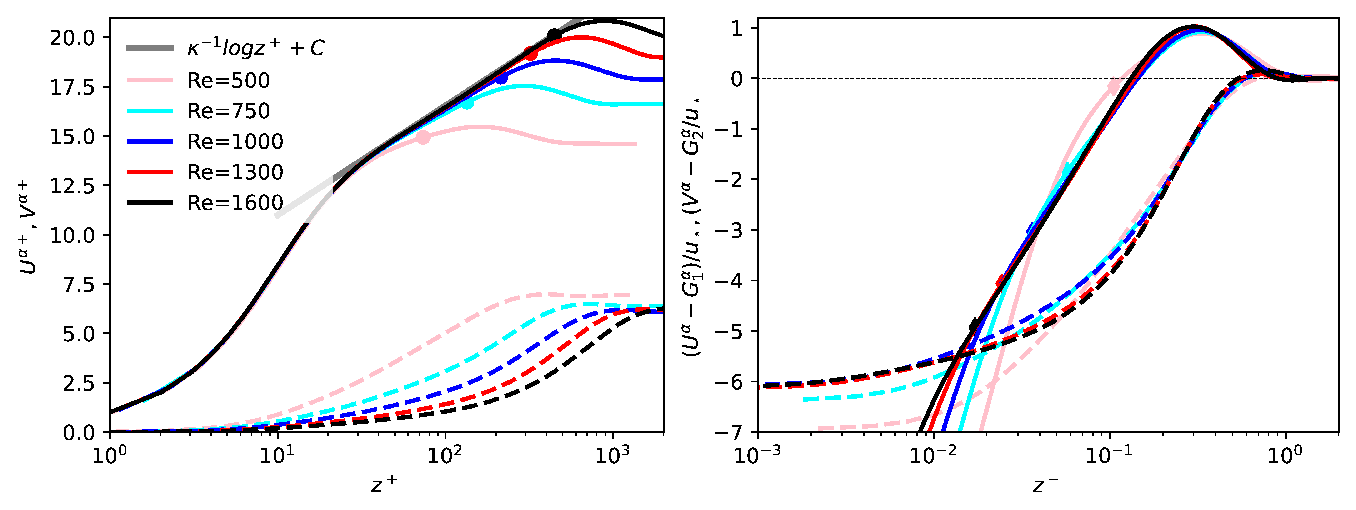
\includegraphics[width=\textwidth]{Fig1.eps}\\ %uv_innerouter.eps}\\
    \caption{
      \textbf{a)} Shear-aligned velocity profiles in inner units; circles mark the
      height $z^-=0.15$;
      \textbf{b)} Shear-aligned velocity deficit in outer units; diamonds mark the grid point closest to the height $z^+=50$
      \label{fig:profiles}
    }
  \end{flushleft}
\end{figure}

\begin{figure}
  \textbf{a)}\hspace{0.47\textwidth} \textbf{b)}\\
  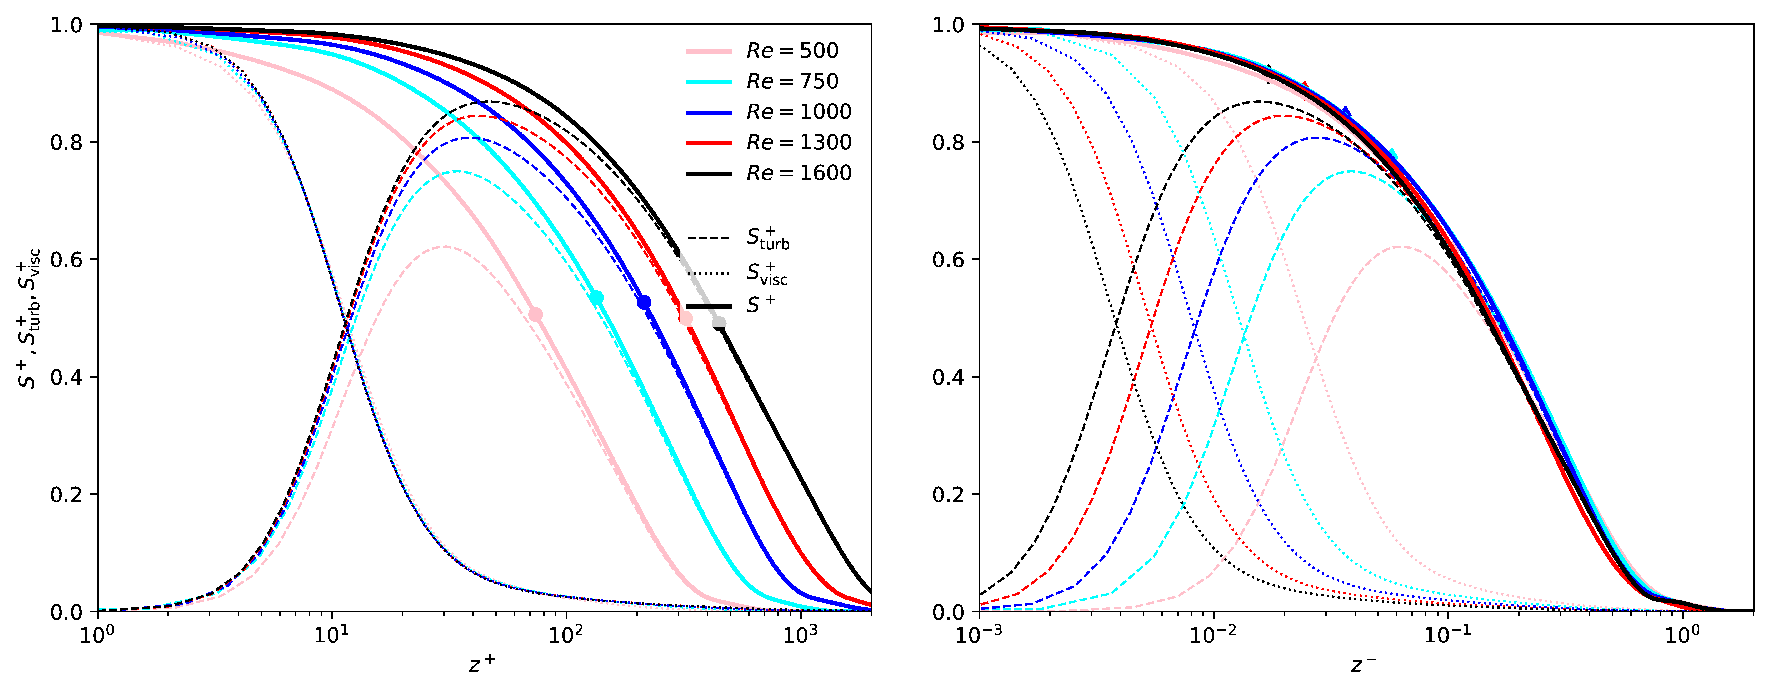
\includegraphics[width=\textwidth]{Fig2ab.eps}\\  %stresses.eps}
  \textbf{c)}\hspace{0.47\textwidth} \textbf{d)}\\    
  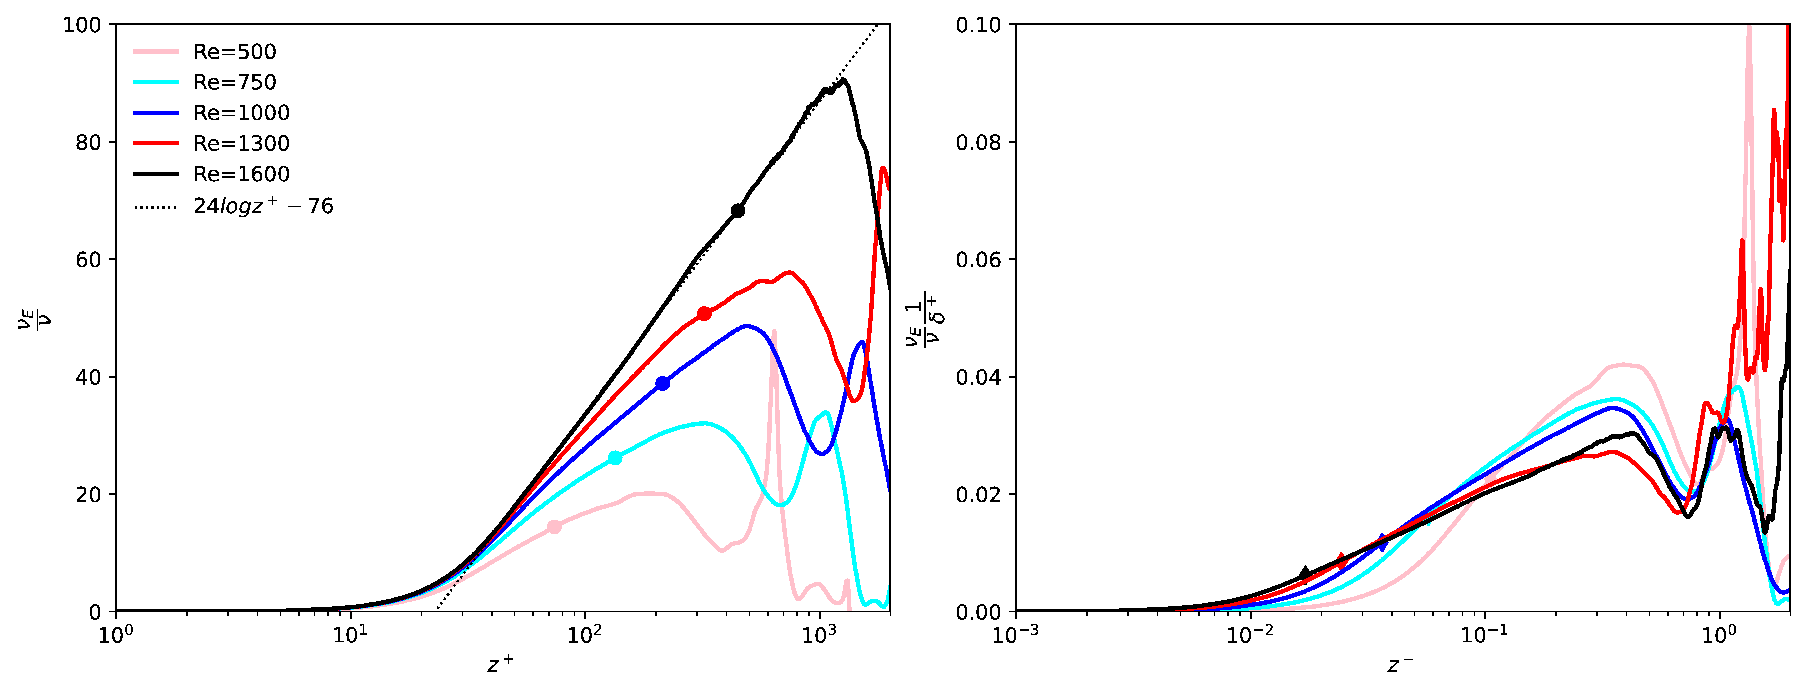
\includegraphics[width=\textwidth]{Fig2cd.eps}\\ %-eddy_viscosity.eps}\\
  \caption{
    \textbf{a-b)} Profiles of
    the turbulent stress $S_\mathrm{turb}^+$ (dashed), 
    the viscous stress  $S_\mathrm{visc}^+$ (dotted), 
    and the total stress, $S^+=S_\mathrm{visc}^++S_\mathrm{turb}^+$ (solid)
    as a function of inner height \textbf{(a)} and outer height \textbf{(b)}. 
    \textbf{c-d)} Normalized eddy viscosity $\nu_E$ (solid) plotted versus
    inner height \textbf{(c)} and outer height \textbf{(d)}. \textbf{(c)} uses inner normalization; 
    \textbf{(d)} uses normalization by $\nu \delta^+$ which approximately collapses data in the 
    outer layer. 
    Different colors are for different Reynolds numbers (cf. Tab.~\ref{tab:sim-setup}).
    Circles in \textbf{(a)} and \textbf{(c)} denote the height
    $z^-=0.15$, diamonds in \textbf{(b)} and \textbf{(d)} are for $z^+=50$
    as in Fig.~\ref{fig:profiles}
    \label{fig:stresses}} 
\end{figure} 
The viscous stress
%
\begin{subequations}
\begin{equation}
  S_\mathrm{visc}= \nu \sqrt{\left(\frac{\p U}{\p z}\right)^2  + \left(\frac{\p V}{\p z}\right)^2}
\end{equation}
exhibits universal scaling when considered as $S_\mathrm{visc}^+(z^+)$ (Fig.~\ref{fig:stresses}a); this normalization is also appropriate in the outer layer where the viscous stress
is, however, small. 
%
Small deviations from the universal profile are observed for the smallest Reynolds number $\RE=500$; 
we attribute these to low-$\RE$ effects in the only transitionally turbulent flow ($\RE_\tau=479$). 
%
In contrast to the viscous stress, the total stress follows outer normalization, i.e.
$S^+(z^-)$ is universal; a discrepancy in the inner layer does not occur as the total stress
is approximately constant in the viscous and buffer layer, and a rescaling of the height would have
no effect there; above, outer scaling is appropriate for the well-established dynamics 
in the overlap region of inner and outer layer.
%
This, however, implies a mixed scaling for the turbulent stress, 
\begin{equation}
  S_\mathrm{turb} = \sqrt{\overline{u' w'}^2 + \overline{v'w'}^2}, 
\end{equation} 
where dashed quantities $u'$, $v'$, $w'$ indicate deviations from the mean and the overbar denotes 
horizontal and time averaging. 
%
Indeed, $S_\mathrm{turb}$ only follows inner normalization below $z^+\lesssim 20$
(where the turbulent contribution is negligible).
%
In the outer layer, where $S_\mathrm{visc}\rightarrow 0$, $S_\mathrm{turb}^+$
follows outer normalization for $z^-\gtrsim0.15$---with increasing accuracy for larger $\RE$ and larger distance from
the surface. 
%
In the overlap region, i.e. for $z^+>20$ and $z^-<0.15$, the mixed scaling for the
turbulent stress can be expressed as
\begin{equation}
  S_\mathrm{turb}^+(z^+,\RE_\tau) = S^+(z^-) - S_\mathrm{visc}^+(z^+), 
\end{equation}
\end{subequations} 
where $z^-=z^+/\RE_\tau$. 
%
\par
%
The eddy viscosity plays a crucial part when modelling profiles and the vertical
transport in turbulent flow. 
%
In analogy to the Fick-law for molecular diffusion, the eddy diffusivity is
the effective diffusivity that yields the turbulent transport $S_\mathrm{turb}$ based
on the strain rate.
%
For the assumptions of horizontal homogeneity and incompressibility (which implies  $W=0$, i.e. no mean wall-normal velocity), it is
%
\begin{subequations} 
\begin{equation}
  \nu_{E}= \frac{S_\mathrm{turb}}{\sqrt{\left(\frac{\p U}{\p z} \right)^2 + \left(\frac{\p V}{\p z}\right)^2}} = \nu \frac{S_\mathrm{turb}}{S_\mathrm{visc}}.  
\end{equation}
%
The inner normalization of $\nu_E$ is obtained when dividing by the molecular viscosity:
\begin{equation}
  \nu_E^+=\nu_E/\nu = S_\mathrm{turb}/S_\mathrm{visc}.
\end{equation}
%
Under this normalization, the profiles of eddy viscosity collapse below $z^+\approx 20$ with a tendency towards better collapse
at higher $z^+$ for higher Reynolds number (up to $z^+\approx 50$ for $\RE=1600$; Fig.~\ref{fig:stresses}c).
%
In the outer layer, the eddy viscosity is characterized by a distinct minimum at $z^-\approx 0.6-0.8$,
and we find that the following mixed normalization of $\nu_E$ by the geostrophic wind and friction velocity
collapses the value of $\nu_E$ at this minimum (cf. Fig.~\ref{fig:stresses}d): 
%
\begin{eqnarray}
  \nu_E^-=\nu_E^+  \frac{1}{\delta^+} = \nu_E \frac{1}{\nu} \frac{\nu}{u_\star \delta}  = \nu _E \frac{f}{u_\star^2}.
  \label{eqn:evisc_outer_scaling}
\end{eqnarray}
\end{subequations} 
%
Substantial variation of the profiles is, however observed below and above this minimum for
different $\RE$ which illustrates that this normalization is probably not generally appropriate
across the outer layer.
% 
\par
%
\begin{figure}
  \centerline{
    \includegraphics[trim=0 0 1152 0, clip, width=0.33\textwidth]{Fig3a.png}
    \includegraphics[trim=1152 0 0 0, clip, width=0.33\textwidth]{Fig3b.png}
    \includegraphics[trim=0 0 1152 0, clip, width=0.33\textwidth]{Fig3c.png}}
  \centerline{
    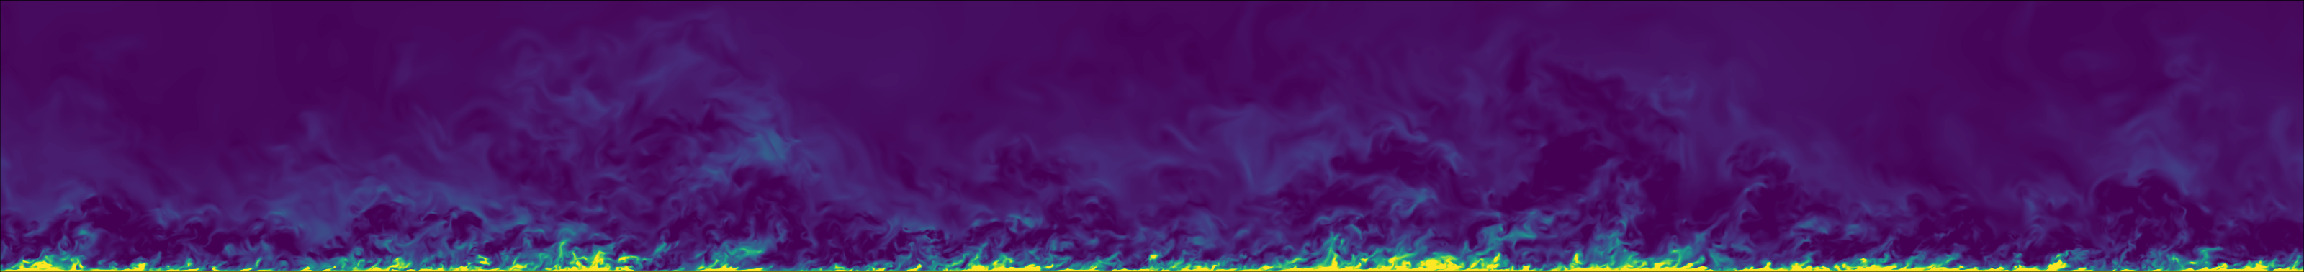
\includegraphics[trim=1152 0 0 0, clip, width=\textwidth]{Fig3d.png}}
  \caption{Horizontal slices of turbulence kinetic energy in the
    Buffer layer (i=10, $z^+\approx 10.5$),
    logarithmic layer (i=100, $z^+ \approx 150$), and
    outer layer (i=400, $z^+ \approx 1200$) of the case with $Re_\tau=2978$;
    coloring between percentiles 4 and 96 of the respective image. Lower panel:streamwise--vertical intersect through the domain 
    \label{fig:slices}}
  
\end{figure} 
The organization of the flow with $Re_\tau=2978$ is depicted in terms of the turbulence kinetic energy in Fig.~\ref{fig:slices}.
%
In vicinity of the wall, at $y^+\approx 10$, (Fig.~\ref{fig:slices}a), elongated streaks aligned with the
surface shear stress dominate.
%
Moving away from the wall, to $y^+\approx 150$ (well within the logarithmic region), the structures
are larger and more isotropic, but they are still largely aligned with the surface shear stress.
%
In the upper part of the outer layer, around $y^+\approx 1000$, no clear signature of the
surface veering direction is found, and intense TKE structures (bright yellow)
are organized on a large spatial scale with weaker eddies (greenish structures) and quiescent regions
in between.  

%%%%%%%%%%%%%%%%%%%%%%%%%%%%%%%%%%%%%%%%%%%%%%%%%%%%%%%%%%%%%%%%%%%%%%%%%%%%%%%%
\section{A Reynolds-number-independent velocity profile for the turbulent Ekman layer}
\label{sec:profiles} 
%%%%%%%%%%%%%%%%%%%%%%%%%%%%%%%%%%%%%%%%%%%%%%%%%%%%%%%%%%%%%%%%%%%%%%%%%%%%%%%%
%
We now turn to the formulation of a general velocity profile that is fully determined by the only
parameter of the idealized problem, namely a Reynolds number representing the scale separation or
geometric size of the problem.
%
This precludes, first, a drag law wherewith we begin this section (\ref{sec:drag-law}).
Based on the scaling arguments put forward in Sec.~\ref{sec:scaling}, we then develop, second,
a formulation of the wind vector in the Ekman layer (Sec~\ref{sec:ekman}). Finally, we come up
with a separate formulation of the, third, stream-wise and, fourth, span-wise velocity components in the
overlap and inner regions of the flow. 
%
% 
\subsection{Drag-law}
\label{sec:drag-law}
\begin{figure}
  \centerline{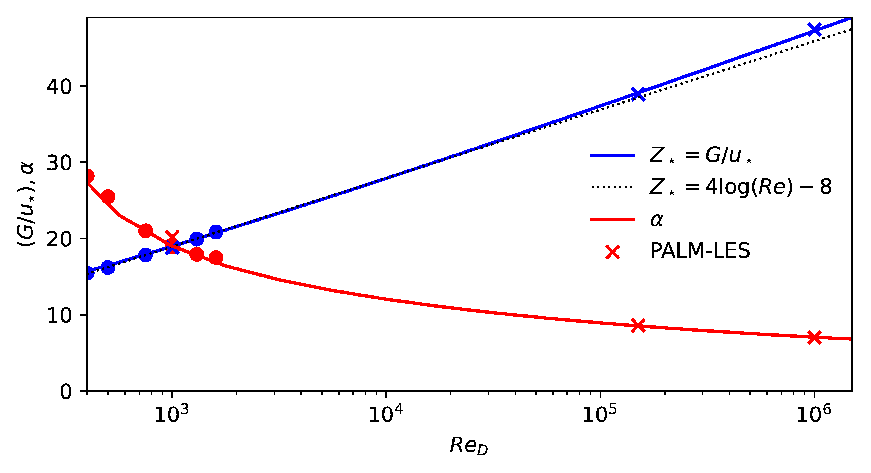
\includegraphics[width=0.7\textwidth]{Fig4.eps}} % ustar_alpha.eps}}
  \caption{Variation of geostrophic drag, $Z_\star$, and surface veering, $\alpha_\star$, with Reynolds number according to
    the theory by Spalart et al. (1989) and as estimated from DNS data
    \label{fig:drag_law}}
\end{figure}
A drag-law for Ekman flow determines---as a function of Reynolds number alone---the surface drag.
%
This can be formulated by the normalized surface friction, $u_\star$ (Eq.~(\ref{eqn:ustar_def}), also termed geostrophic drag), 
and the direction of surface shear stress, $\alpha_\star$ (Eq.~(\ref{eqn:alpha_def}), also termed wind veer). 
%
A non-zero veering of the wind is a rather special case in comparison with most turbulent flows considered in an
engineering context, and it confronts us with a situation where the most appropriate coordinate system
for analysis (namely that aligned with the surface shear stress) is a priori unknown. 
%
We compare our DNS data against a semi-empirical drag-law based on integral consideration \citep{spalart:JFM1989}
and find, as demonstrated in previous work \citep{ansorge:BM2014}, excellent agreement in the range
 $400<\mathbf{Re}<1600$, representing a factor of 16 in variation of viscosity. 
%
\par
%
We also find that the solution of the transient equation involved in estimation of $u_\star$ for a given Reynolds number
$Re_D$ is approximated reasonably by the formulation
\begin{equation}
  Z_\star= 4\log(\mathbf{Re}_D))-8
  \label{eqn:zstar}
\end{equation}
which quantifies the 'weak' dependence of $u_\star$ on the Reynolds number as an approximately logarithmic one, at least
for problems with a scale separation on the order that is relevant to geophysical problems ($Re_D<10^{8}$).  
%
%%%%%%%%%%%%%%%%%%%%%%%%%%%%%%%%%%%%%%%%%%%%%%%%%%%%%%%%%%%%%%%%%%%%%%%%%%%%%%%%
%
\subsection{Profile in the Ekman layer}
\label{sec:ekman}
%
Formulations for the outer layer that take into account the rotation
(and thus deviation from the channel-flow analogy)
need to be matched to the framework of surface similarity.
%
A smooth transition from the inner layer to the Ekman layer, where the wind is characterized by a turning
of its mean direction, is not easily achieved. 
%
\cite{optis:BM2014}, for instance, define an \emph{``effective geostrophic wind vector that has the same magnitude of the
observed surface geostrophic wind and is rotated by the angle $\alpha$ [their nomenclature]''} to overcome the
unsteady transition when approaching the Ekman layer from below.
%
Such rotation of the wind vector is \emph{a posteriori} justified by the observational data that the model outcomes are compared to.
%
This need for a connection of the two reference frames is a manifestation of a
mismatch in the theoretical treatment of the inner and outer layer in this rotating flow configuration. 
%
\par
%
The text-book solution for Ekman flow makes use of the physical boundary conditions (BCs) for
the~ABL (no-slip at the bottom and geostrophic wind in the free atmosphere) and a constant eddy
viscosity.
%
Specifying the boundary conditions at top and bottom eliminates one mode of the analytical solution, and
it determines the magnitude of the spiral.
%
In doing so, one has to assume that the solution is appropriate across the entire ABL, which is not the case:
The dynamics put forth by \citeauthor{ekman:AMA1905} in \citeyear{ekman:AMA1905}
are not appropriate in the surface layer of the ABL; better approximations exist for the logarithmic,
buffer, and viscous sublayers. 
%
In view of this situation, we use an adapted Ekman spiral that does not enforce the
boundary conditions at the surface but at a different height while maintaining the restriction 
to constant eddy viscosity. 
%
This is achieved by considering the Ekman spiral only in the Ekman layer,
thus giving way for the well-established logarithmic and viscous-layer profiles in the
lower surface layer. 
%
Based on the derivation in App.~\ref{app:ekman_solution}, this profile is given by 
\begin{subequations}
  \label{eqn:profile_ekman}
  \begin{eqnarray}
    \frac{1}{G}\left(\begin{array}{c} 
      U_\mathrm{ek}\\ 
      V_\mathrm{ek}
    \end{array}\right)  &=& \left(\begin{array}{c} 1 \\ 0 \end{array}\right) 
    + e^{-z_\mathrm{ek}} \left[ a_\mathrm{ek}  \left(\begin{array}{r}
      -\cos z_\mathrm{ek} \\ 
      \sin z_\mathrm{ek}
      \end{array}\right)  + b_\mathrm{ek}\left(\begin{array}{r}
        \sin z_\mathrm{ek} \\ \cos z_\mathrm{ek}
        \end{array}\right)\right]. 
  \end{eqnarray}
\end{subequations}
with  $z_\mathrm{ek} = \delta_\mathrm{ek} (z^- -s_\mathrm{ek})$.
% 
The right-hand-side consists of two modes with magnitude $a_\mathrm{ek}$ and $b_\mathrm{ek}$
shifted by $\pi/2$ with respect to each other. 
%
In the classic case, the second mode governed by $b_\mathrm{ek}$ is incompatible with
the surface boundary condition. 
%
While this is not the case here for the general form of the profile, the
phase shifts can also be captured by the parameter $s_\mathrm{ek}$, 
and we stick with to a single-modal approach, i.e., we let $b_\mathrm{ek}=0$. 
%
\par 
%
This single-modal solution is characterized by three parameters,
(i) an Ekman-layer depth scale $\delta_\mathrm{ek}$,
(ii) the magnitude parameter of the spiral $a_\mathrm{ek}$, and
(iii) a zero-crossing point for the velocity $s_\mathrm{ek}$.
%
The effects of varying these parameters are illustrated in Fig.~\ref{fig:ekman_ideal} where
the classic Ekman solution is recovered by setting $a_\mathrm{ek}=1$, $s_\mathrm{ek}=0$ and
$\delta_\mathrm{ek}=\sqrt{2\nu/f}$.
% 
These parameters are \emph{a priori} unknown as they need to conform to the turbulent state of the
boundary layer; we use our DNS data to arrive at best estimates for them.
%
\par
%
\begin{figure}
  \begin{flushleft}
    \textbf{\ \ a)}\hspace{0.45\textwidth}\textbf{\ \ b)}\\
  \end{flushleft} 
  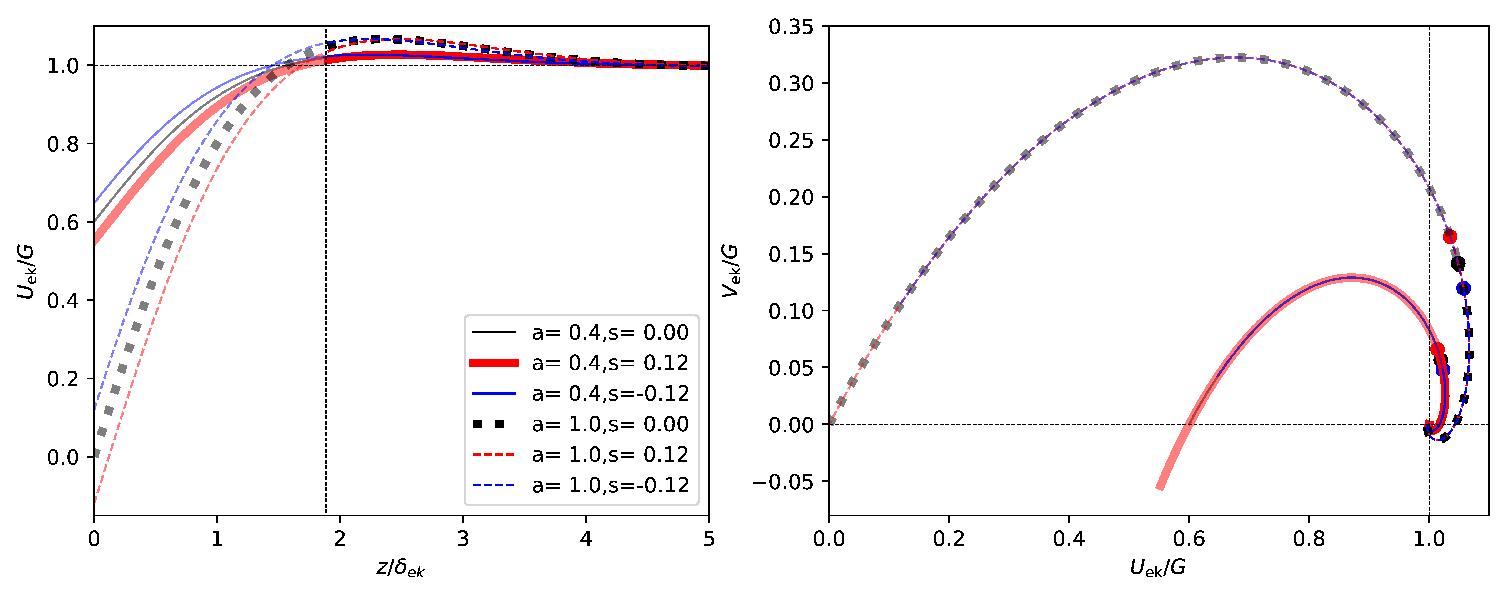
\includegraphics[width=\textwidth]{Fig5.eps} %ekman_ideal.eps}
  \caption{\label{fig:ekman_ideal}
    \textbf{a)} Generalized Ekman-profile of the geostrophic-aligned component $U_\mathrm{ek}$.
    \textbf{b)} Hodograph for the geostrophic-aligned and pressure-gradient aligned components $U_\mathrm{ek}$ and $V_\mathrm{ek}$.
    Thick, black dashed line shows the classic solution. The height corresponding to $z^-=0.30$ is marked by the dashed line in panel \textbf{(a)}
    and by filled circles in panel \textbf{(b)}. The hodograph and profiles above this reference height are
    shown as solid lines, below as opaque line.
  } 
\end{figure} 
%
\textbf{The Ekman-layer depth scale} $\delta_\mathrm{ek}$ is fundamentally defined by the eddy viscosity.
%
However, we have seen in Section \ref{sec:scaling} that a characteristic value for the eddy diffusivity
is not easily obtained for its strong dependence on the Reynolds number and distance from the surface.
%
We therefore resort to the physical manifestation of the eddy diffusivity in an Ekman layer, and use the
boundary layer depth $\delta_\mathrm{ek} = 0.66 \delta \times 2\pi$.
%
For the relation $\delta_\mathrm{ek}=\sqrt{2\nu_\mathrm{ek}/f}$, this yields
$\nu_\mathrm{ek} \propto u_\star^2/f$ in accordance with the observations in
Sec.~\ref{sec:scaling} (Eq.~\ref{eqn:evisc_outer_scaling}). 
%
\par
%
\textbf{The magnitude parameter of the Ekman spiral}, $a_\mathrm{ek}$, defines the super-geostrophic maximum of the
wind profile aloft the logarithmic layer. Our simulations suggest this maximum of the velocity deficit
remains constant when normalized by $u_\star$ as shown in Fig.~\ref{fig:profiles_outer}.
%
The numerical value of $a_\mathrm{ek}$ is estimated from visual comparison, and we find $a_{ek}=8.4u_\star$;
while this appears rather large, it is pre-multiplied by $e^{-z_\mathrm{ek}}$ which has already decreased
to $\mathcal{O}(0.1)$ at the height of this maximum.
%
This choice ascertains that the velocity deficits $U/u_\star-Z_\star$ and $V/u_\star-Z_\star$ do not
depend on the velocity scale $u_\star$, but only on $G$ as
\begin{equation}
  U_\mathrm{ek}/u_\star-Z_\star \propto a_\mathrm{ek} Z_\star = 8.4G.
  \label{eqn:hodograph_scaling}
\end{equation}
%Thus, the reduction of the area under the Ekman hodograph is directly linked to the variation
%in the friction velocity, which quantifies the well-known qualitative observation that a more turbulent boundary
%layer leads to a flatter hodograph in Ekman flow.
%
\par
%
\textbf{The offset parameter} $s_\mathrm{ek}$ defines the zero-crossing height of the profile
(in contrast to $\delta_\mathrm{ek}$, which determines the thickness across which the wind veering takes place). 
%
Physically, this offset can be understood as the height at which the surface was located assuming
a perfect Ekman flow down to the surface.
%
As this is not the case, and gradients are steeper in the highly turbulent boundary layer flow encountered
when approaching the surface, the offset is smaller than zero (the fully turbulent boundary layer is
actually thinner than an Ekman layer would be).
%
From our DNS data, we estimate $s_\mathrm{ek}=-0.12$. 
%
\par 
% 
In summary, the outer layer of Ekman flow is characterized by a turning of the wind
velocity and the super-geostrophic maximum that is sustained by momentum convergence
at the inflection point of the velocity profile.
%
The super-geostrophic maximum of streamwise velocity and a secondary minimum aloft the bulk-turbulent part of
the boundary layer are well-described by a classic Ekman spiral with adapted boundary conditions and a shift
in reference height.
%
While alternative approaches exist that incorporate a variation of the eddy viscosity \citep{basu:BM2023}, 
we stick here to \citeauthor{ekman:AMA1905}'s classic assumption of constant eddy viscosity. 
As the Ekman spiral is applied only for $z>z_{blend}\approx 0.28$ (cf. Sec.~\ref{sec:matching}
below), the assumption of constant eddy viscosity is also weakened in the sense that it is only required for 
$z>z_{blend}$. 
% 
Corresponding profiles are shown in comparison with data from three DNS runs in Fig.~\ref{fig:profiles_outer}.
The idealized profiles capture the secondary minimum and convergence to the geostrophic equilibrium in the
non-turbulent flow very well.
%
Deviations from the Ekman spiral are found towards the lower end of the corresponding height range, 
marked by a dot in the figure; this is consistent with an increasing variation of eddy viscosity when 
the more turbulent part of the boundary layer is entered from aloft. 

\begin{figure}
  \begin{flushleft}
    \textbf{\ \ a)}\hspace{0.45\textwidth}\textbf{\ \ b)}\\
  \end{flushleft} 
  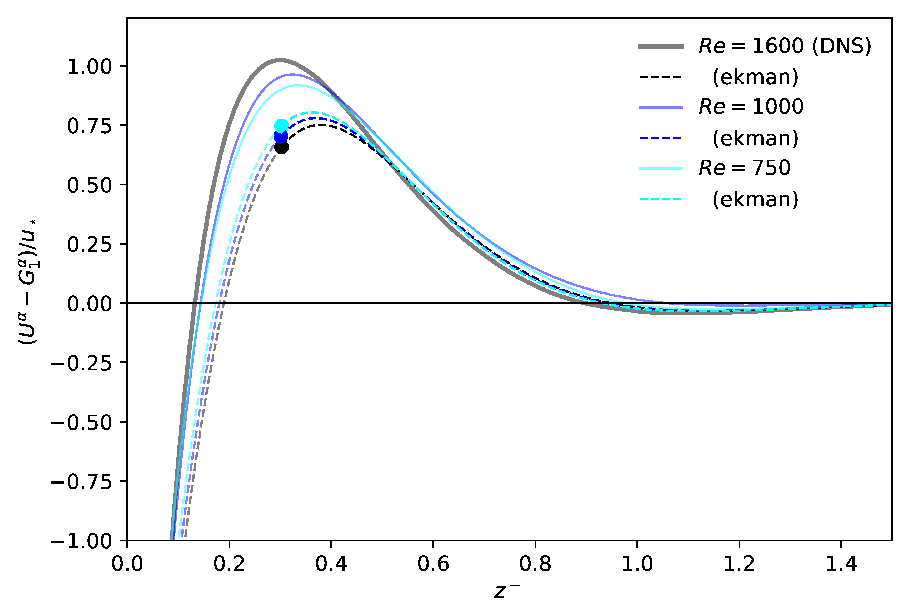
\includegraphics[width=0.5\textwidth]{Fig6a.eps} %outer_layer_u.eps}
  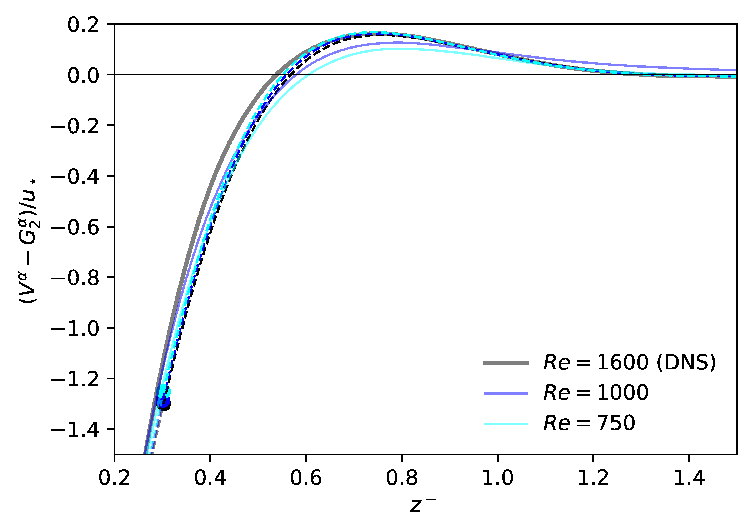
\includegraphics[width=0.5\textwidth]{Fig6b.eps} %outer_layer_w.eps}
  \caption{
    \label{fig:profiles_outer}
    Shear-aligned velocity deficit for the streamwise (panel \textbf{(a)}) and spanwise (panel \textbf{(b)})
    components of the mean velocity $U^\alpha$ and $V^\alpha$.
    Solid lines show DNS data, dashed lines the Ekman profiles $U_\mathrm{ek}$ and $V_\mathrm{ek}$ as defined in
    Eq.~\ref{eqn:profile_ekman}. 
    %Region below $z^-=0.3$ is shown opaque. 
    Variations in $U_\mathrm{ek}$ and $V_\mathrm{ek}$ are
    a consequence of the normalization and related to changes in $u_\star$ and $\alpha_\star$ among the different $\RE_D$. 
  }
\end{figure}

\subsection{Streamwise velocity component}
\label{sec:streamwise} 
Well-established theories exist for the streamwise velocity profile, which in non-rotating flows is aligned with the surface shear stress due to the geometry. These theories cover various regimes based on their distance from the wall and the relative influence of viscosity, turbulence, and interaction with the outer flow region, with the logarithmic law for the mean velocity serving as a central reference point.
%
\par
%
\begin{subequations}

In immediate vicinity to the surface, local turbulent mixing cannot occur for the no-slip/no-penetration boundary condition,
and the mean velocity is described by a viscous profile of the form
\begin{equation}
  U^{\alpha_\star+}  = z^+
\end{equation}
where the direction of the velocity points into the exact opposite direction of the wall shear stress $\tau$. 
In absence of roughness elements and for small roughness ($z_0^+<5$), this linear regime is known as
viscous sub-layer \cite{foken:m2002,foken:BM1978}.
%
In fact, this law of the wall has no degree of freedom given the drag, i.e. once $u_\star$ and $\alpha_\star$ are defined. 
%
However, theoretical foundation is lacking for the exact shape of the velocity profile in the buffer layer; though crucial for turbulence
production, it is commonly understood as a transition region between the linear profile at the surface and the logarithmic profile
aloft.
A pure blending from the linear velocity profile into the logarithmic one is, however, not reasonable as both the linear and logarithmic
profile overestimate the velocity in the buffer layer.
%
We therefore introduce a two-step correction procedure, accounting for the smaller-than linear growth beyond $z^+\approx 5$, and assuring smooth matching with the logarithmic law at $z^+=40$:
\begin{equation}
  U_\text{inner}^{{\alpha_\star}^+} = \frac{z^+}{1+c_1 (y^+)^2} +  (c_2 z^+ - a_\mathrm{match} )\frac{1+tanh\left[0.2(z^+-22)\right]}{2} + c_3 e^{-c_4(z^+-22)^2}. \label{eqn:u_inner} 
\end{equation} 
%
We use here
\begin{equation*}
  c_1 = 0.00185;\quad
  c_2 = 0.195;\quad 
  c_3 = 0.4 ; \quad
  c_4 = 0.35. 
\end{equation*}
%
The second and third terms on the right hand side vanish for $z^+\ll 22$, and $c_1=0.00185$
implies an approximately 5\% correction at $z^+=5$ and an 18.5\% correction at $z^+=10$.
%
The second and third term on the R.H.S. of eq.~(\ref{eqn:u_inner}) are an empirical fit to
the velocity profiles observed in the buffer layer and appear independent of the Reynolds number
for the range observed here.
%
The coefficient $a_\mathrm{match}$, which has no effect in the viscous sublayer, is then used to
match this formulation to the logarithmic law employed above. 
%
\par
%
In the logarithmic region, we use the profile
\begin{equation}
  {U_\text{log}^{\alpha_\star}}^+ = \frac{1}{\kappa} \log z^+ + C 
\end{equation}
with the von-K\'arm\'an constant $\kappa=0.416$ and the boundary condition $C=5.4605$. %  log-layer (K\'arm\'an, Prandtl, Jimenez, Marusic)
For this logarithmic law, $a_\mathrm{match}=3.569861$ for a matching at $z^+=40$. 
%
\par %%%%%%%%%%%%%%%%%%%%%%%%%%%%%%%%%%%%%%%%%%%%%%%%%%%%%%%%%%%%%%%%%%%%%%%%%%%%%%%%
%
\end{subequations} 
%
\begin{figure}
  \begin{flushleft}
    \textbf{\ \ a)}\hspace{0.45\textwidth} \textbf{\ \ b)} 
  \end{flushleft} 
  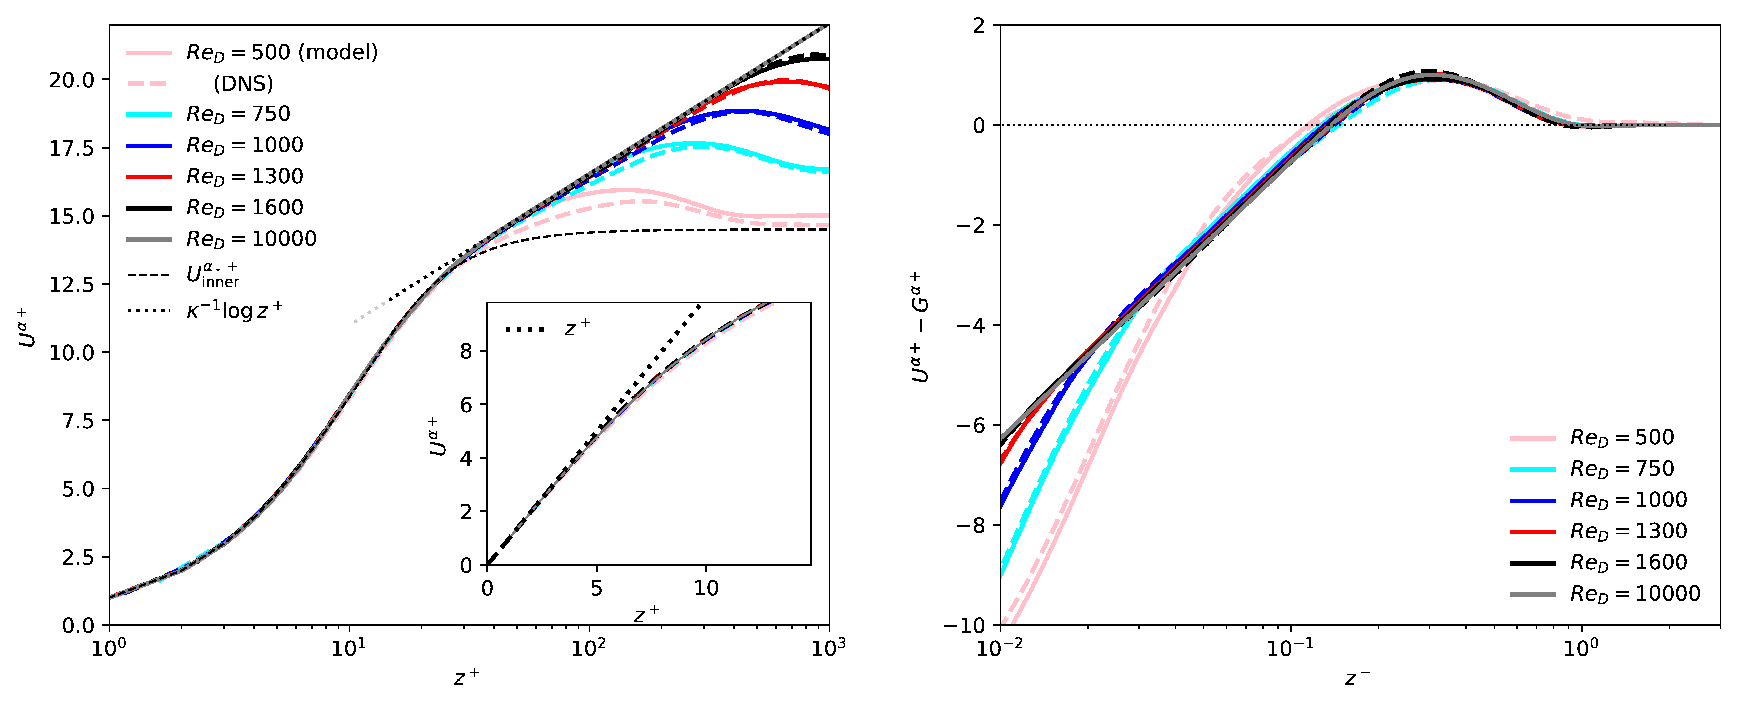
\includegraphics[width=\textwidth]{Fig7.eps} % u_profile.eps}
  \caption{Shear-aligned profiles of velocity components $U^{\alpha_\star+}$ in inner (left) and outer (right) units.
    \label{fig:u_profiles}} 
\end{figure} 
%
%%%%%%%%%%%%%%%%%%%%%%%%%%%%%%%%%%%%%%%%%%%%%%%%%%%%%%%%%%%%%%%%%%%%%%%%%%%%%%%%%%%
%
\subsection{Spanwise velocity component}
\label{sec:spanwise} 
%
%%%%%%%%%%%%%%%%%%%%%%%%%%%%%%%%%%%%%%%%%%%%%%%%%%%%%%%%%%%%%%%%%%%%%%%%%%%%%%%%%%%
%
The background rotation and associated veering of the surface wind implies a non-zero profile for the span-wise
velocity which challenges the conventional assumptions related to the channel-flow analogy:
%
While the analogy with channel flow in vicinity of the wall implies that the streamwise component
be zero or at least small, the veering requires a value of $V_{top}=U_G\sin\alpha_\star$ in the free stream
(and thus also at the top of the boundary layer if we assume that any substantial velocity gradient is
confined to the turbulent part of the flow). 
%
This continuous rotation of the wind vector is conveniently visualized by velocity hodographs
aligned with the outer, geostrophic flow (cf. Fig.~\ref{fig:ekman_ideal}b) and normalized by
the geostrophic wind. 
%
The geometry of the flow and its drag imply the following for any hodograph: 
(i) the boundary conditions at the surface,
(ii) the boundary condition at the top, and
(iii) the inclination of the hodograph at the origin by the surface veering:
\begin{subequations} 
\begin{eqnarray} 
  V^{\alpha_\star}(z=0) &=& 0,\\ 
  \lim_{z\rightarrow\infty} V^{\alpha_\star} &=& G \sin\alpha_\star \\ 
  \left.\partial_{z^+} V^{\alpha_\star+}\right|_{z=0} &=& 0.  
\end{eqnarray} 
\end{subequations} 
%
\par
%
Outer scaling of the velocity profile further implies that the velocity deficit of
$(V^{\alpha_\star}-G^{\alpha_\star})/u_\star$ be a universal function of the outer height $z^-$. 
%
In the outer region of the flow (for $z^-\mapsto 1$), $f_V(z^-)$, should govern the
spanwise velocity profile, as is supported by our DNS data (Fig.\ref{fig:profiles}b);
above $z^-\approx 0.3$, this profile is very well approximated by the Ekman-turning derived
above (Eq.~(\ref{eqn:profile_ekman}); Fig.~\ref{fig:profiles_outer}b). 
%
While this deficit is a signature of outer rotation,
it is inappropriate to extend this general relation to the surface where inner
scales matter:
%
On the one hand, the variation of the spanwise velocity deficit across
the boundary layer (i.e. between $0<z^-<1$) must match the difference implied by the drag law ($u_\star, \alpha_\star$)
and the constant value of $V^{\alpha_\star}$ around $z^-=0.3$.
%
On the other hand,--provided the outer velocity deficit is $\RE$ independent--the $\RE$-dependence
of $\alpha_\star$ and $u_\star$ implies that this difference cannot be constant as a function of $\RE$.
%
%\par 
%
We hence ask, how does the span-wise component scale when the surface is approached?
%
Clearly, the spanwise contribution is small in comparison with the streamwise component
throughout much of the layer below $z^-\approx 0.3$. 
%
However, we cannot assume $V=0$ if a smooth matching between the inner and outer layers shall be achieved. 
%
In this context, we first realize that the velocity deficit $(V^{\alpha_\star}-G^{\alpha_\star})/u_\star$
approaches a $\RE$-independent constant around $C_{V0}=Z_\star \sin\alpha=6.1$ at the surface; deviations from
this constant are only found for the lowest Reynolds numbers which is in accordance with
the low-$\RE$ correction suggested by \cite{spalart:JFM1989}.
%
This constrains the wind veer, and it quantitatively shows that the decreasing wall friction manifest in an
increase of $Z_\star$ exactly compensates the decrease of wind turning measured by $\sin\alpha_\star$. 

If the difference across the boundary layer is constant ($C_{V0}$) vs. $\RE$,
the averaged gradient $\partial_{z^+} V^{\alpha_\star+}$ of the spanwise velocity component
must decrease as $1/\delta^+$ with increasing $Re_\tau$. 
%
Hence, it should--at a fixed height--be $V^{\alpha_\star} \propto \left(\delta^{+}\right)^{-1}$.
%
A profile that agrees with the constraints of the profile at the surface
and exploits the dependence of $V^{\alpha_\star}$ on $\delta^+$ is 
\begin{equation}
  V^{\alpha_\star}\frac{\delta^+}{G} = f_{V,\mathrm{visc}}(z^+) = v_\mathrm{ref} \left( \omega_v z^+ -1 + \exp[-\omega_v z^+]\right),
  \label{eqn:scaling_spanwise} 
\end{equation}
where $v_\mathrm{ref}$ controls the magnitude of the profile and $\omega_v$ sets the height at which the profile
transitions into an approximately linear one.
%
We find excellent agreement with the DNS data for $500\le\RE_D\le1600$ below $z^+\approx 15$ with
\[v_\mathrm{ref} = 18.85;  \quad \omega_v=0.2353\]
(cf. Fig.~\ref{fig:inner_w}b). 
%
\begin{figure}
  \begin{flushleft}
    \textbf{\ \ a)}\hspace{0.45\textwidth}\textbf{\ \ b)}\\
  \end{flushleft} 
  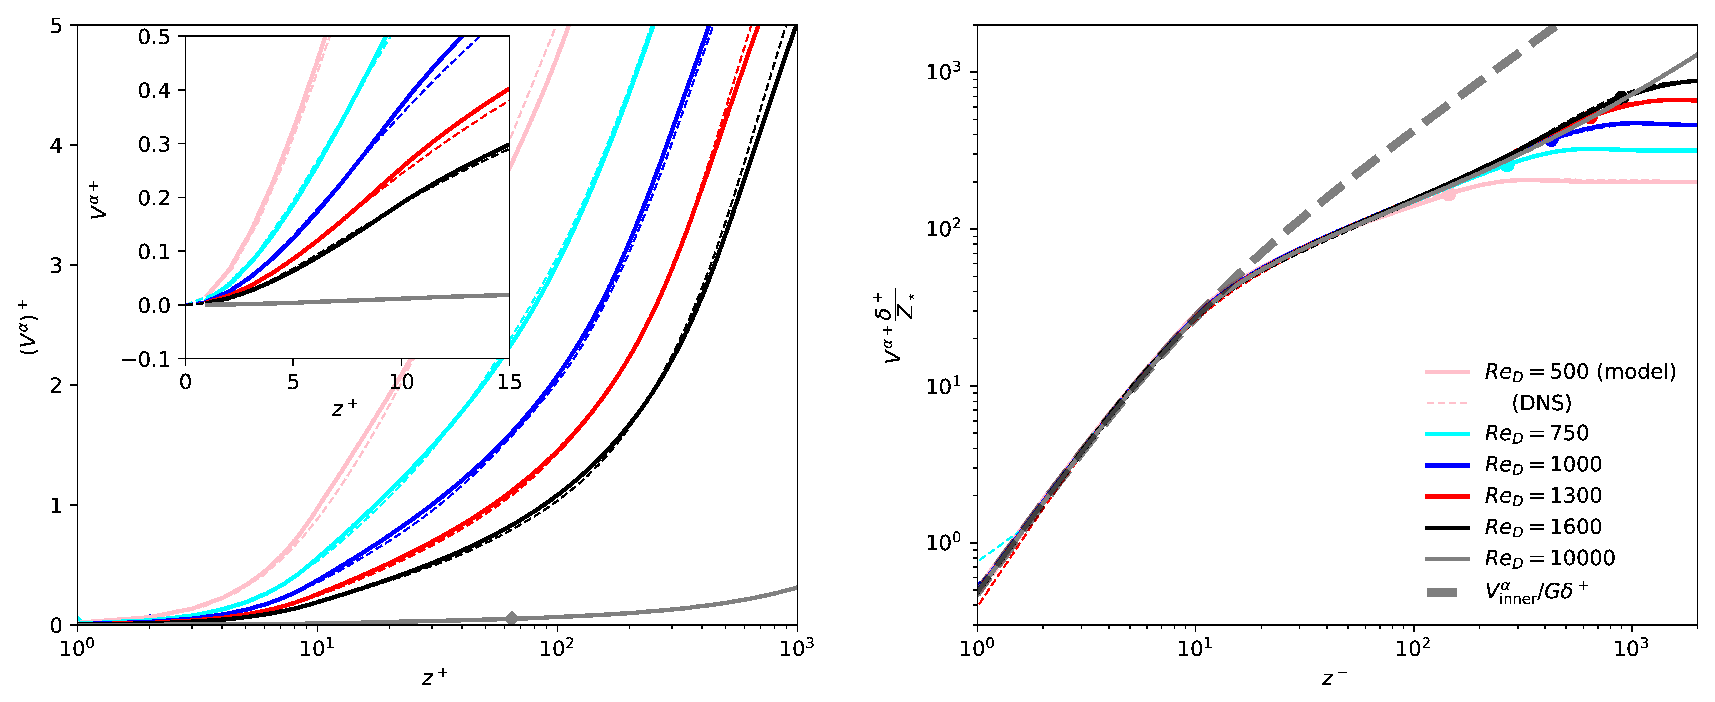
\includegraphics[width=1.0\textwidth]{Fig8.eps} %w_profile.eps}
  \caption{Profiles of shear-aligned span-wise velocity $(V^\alpha)^+$ versus inner height. 
    Dashed lines show DNS data, thick, opaque lines are from the semi-emprical theory developed above.
    Panel \textbf{(a)} shows standard inner normalization, panel \textbf{(b)} the inviscid normalization yielding
    a universal profile for the spanwise component of velocity in the inner layer. }
  \label{fig:inner_w}
\end{figure}
 %
\par
%
For the adjacent surface layer, we find a log-like transition from the quasi-linear profile
inner profile around $z^+=10$ to a linear profile with increasing $\RE$ (Fig.~\ref{fig:inner_w}b).
%
We model this transition by 
%
\begin{equation}
  f_{V,\mathrm{log}}(z^+) = \frac{V_\mathrm{log}(z^+)}{G} \delta^+ = a_\mathrm{log} + b_\mathrm{log} \log z^+ + c_\mathrm{log} z^+. 
  \label{eqn:abc_log}
\end{equation} 
%
This surface-layer profile matches the inner (viscous) scaling in vicinity of the surface to the outer
(Ekman) scaling above $z^-=0.3$ when constrained by the viscous profile at the bottom and the
Ekman profile at the top:
%
\begin{subequations} 
  \label{eqn:match}
\begin{align}
  f_{V,\mathrm{log}}(z^+=10) &=& f_{V,\mathrm{visc}}(z^+=10) &=:& v_{10} \simeq 27.3\\
  \frac{\p}{\p z^+} \left[ f_{V,\mathrm{log}}\right]_{z^+=10} &=& \frac{\p}{\p z^+}\left[ f_{V,\mathrm{visc}}\right]_{z^+=10} &=:&d_{10}\simeq 4.01 \\
  f_{V,\mathrm{log}}(z^+=0.3\delta^+) &=& V^{\alpha_\star}_\mathrm{ek}(z^-=0.3)\delta^+&=:& v_{03} 
\end{align}
\end{subequations}
where $v_{03}$ is determined by $V_\mathrm{ek}(0.3)$ and $U_\mathrm{ek}(0.3)$ and depends on $\RE$.
%
Given the Ekman formulation of the velocity profile introduced in Sec.~\ref{sec:ekman},
one may express $v_{03}$ using the Ekman profile introduced in Sec.~\ref{sec:ekman} together
with the approximation for $u_\star(Re)$ found in Eq.~(\ref{eqn:zstar}). 
% 
%
While the $\RE$-dependency of $a_\mathrm{log}$, $b_\mathrm{log}$, $c_\mathrm{log}$
is small, it shows up in Fig.~\ref{fig:profiles} where the normalized profiles
of spanwise velocity become more convex with increasing $\RE$.
%
We can now quantify this effect by means of the change of $c_\mathrm{log}$ versus $\RE$ which is shown in
Fig.~\ref{fig:clog} (cf. Appendix~\ref{app:log-coefficients};
$a_\mathrm{log}$ and $b_\mathrm{log}$ are then determined by the universal
values of $v_{10}$ and $d_{10}$).
%
%
\begin{figure}
  \centerline{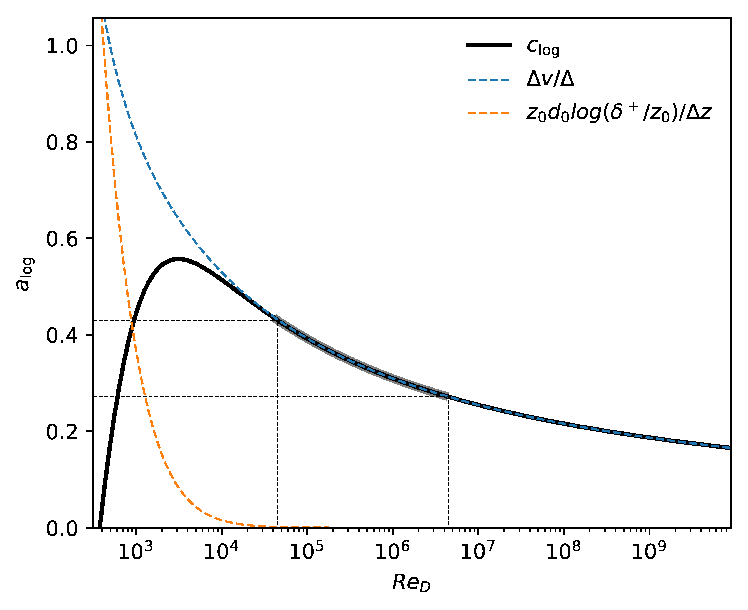
\includegraphics[width=0.5\textwidth]{Fig9.eps}} %c_log.eps}}
  \caption{Coefficients $a_\text{log}$, $b_\text{log}$ and $c_\text{log}$ 
    (cf. Eq.~\ref{eqn:abc_log}) 
    as a function of 
    the viscous Reynolds number $Re_D$. The approximate range of scale separation relevant for atmospheric application 
    is found in between the dotted lines, where $a_\text{log}\simeq 0$ and $c_\text{log}\simeq 0.4$ }
  \label{fig:clog}
\end{figure} 
%
\par
% 
\subsection{Matching of the inner and outer layer profiles}
\label{sec:matching}
% 
The formulations introduced above are continuous across the transition from the inner to 
the outer layer. 
% 
However, the requirement of smooth derivatives would over-constrain the velocity profiles and is hence not applied. 
% 
This can, in particular for low or extremely high $\RE$, cause discontinuity in the derivatives of the velocity profiles around the transition from the inner to the outer layer. 
% 
To avoid such artificial discontinuity, the profiles are blended by an error-function transition using a blending 
height $z_{blend}^-=0.28-2.25\sqrt{1/Re_\tau}$ and a transition thickness 
$z_\text{trans}=2$, 
such that the weighting function $\omega(z^-)$ becomes 
\begin{align}
  \omega(z^-) = \frac12 \left[\text{erf}\left(z_\text{trans}\log\frac{z^-}{z_{\text{blend}}^{-}}\right) +1\right],
\end{align}
hence 
 $u_\text{total} = (1-\omega) \times u_\text{inner} + \omega \times u_\text{outer}$ and similar for $v$. 

%
\begin{figure}
  \phantom{AAA}\textbf{(a)\hspace{0.3\textwidth}(b)\hspace{0.3\textwidth}(c)}\\
  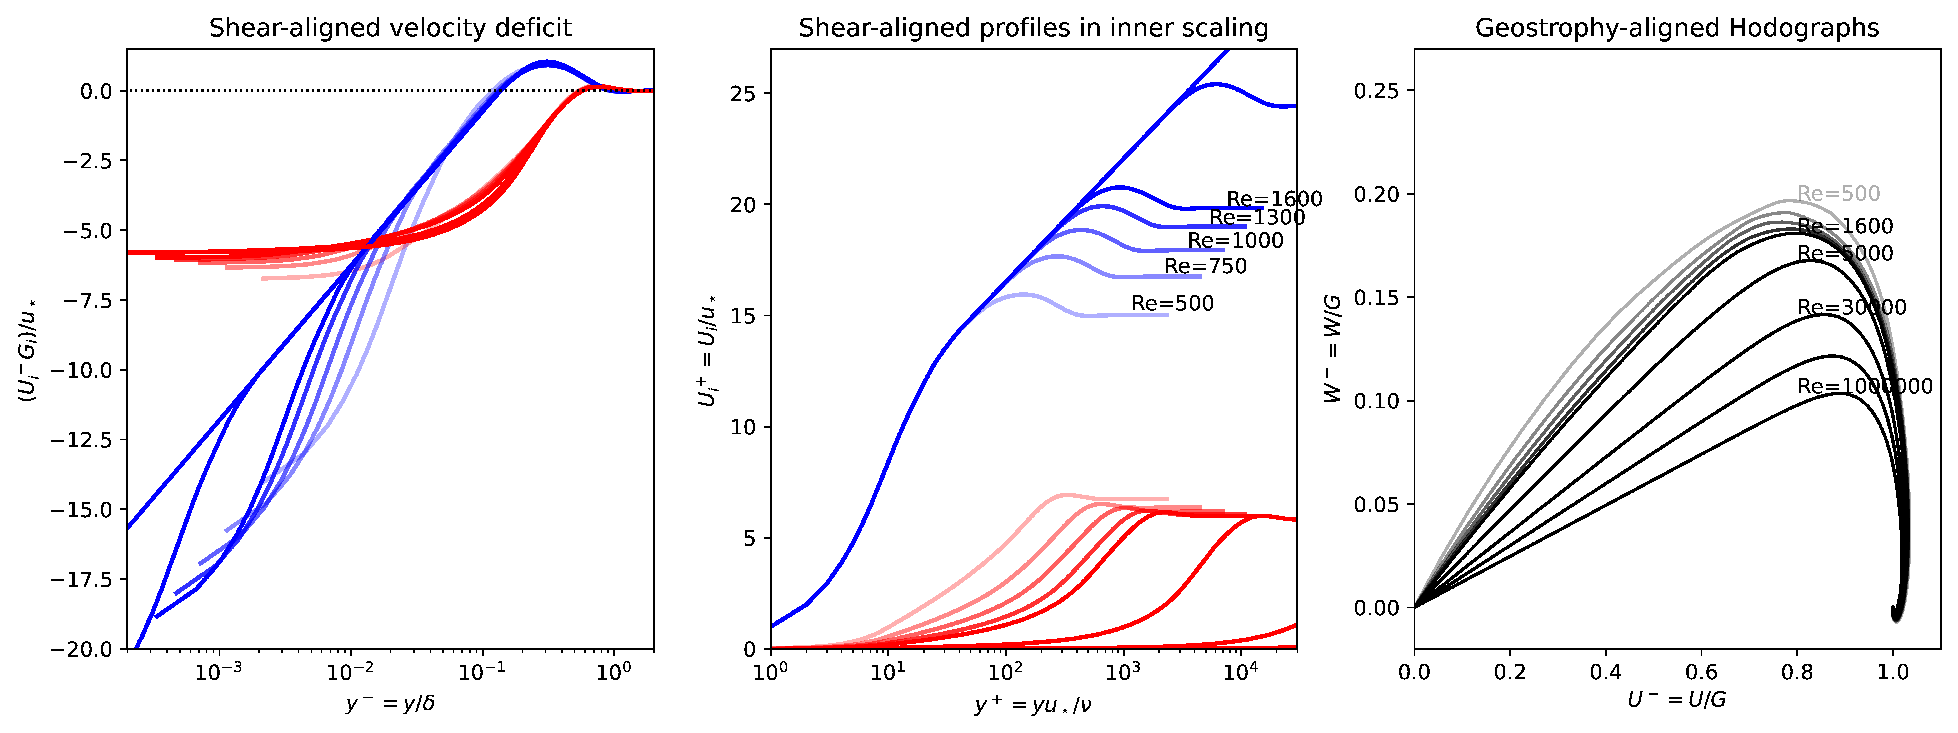
\includegraphics[width=\textwidth]{Fig10.eps}  %ekman_profiles.eps 
  \caption{ \textbf{(a)} Velocity deficit, \textbf{(b)} velocity profile in shear-aligned hodographs and \textbf{(c)} hodograph in geostrophy-aligned coordinates.
   In panels \textbf{(a)} and \textbf{(b)}, blue lines correspond to the streamwise component and red to the spanwise. }
  \label{fig:summary} 
\end{figure} 
The resulting velocity profiles across the entire boundary layer are shown in inner and outer scaling as well as in ho\-do\-graph- view in Fig.~\ref{fig:summary}. The shear-aligned velocity deficit is shown in outer scaling highlighting the universality in the outer layer. 
% 
The logarithmic scaling of the streamwise component is encountered as straight blue lines in panels \textbf{(a)} and \textbf{(b)} where 
the extent of the logarithmic range increases with $\RE$ towards lower values of $z^-$ and higher values of $z^+$ depending on the scaling. 
Importantly, the logarithmic region is widening for increasing Reynolds number -- irrespective of the scaling. 
% 
In this simple inner scaling, the spanwise velocity (which follows a mixed scaling) 
does not collapse but seems to depend on $Re$ (the collapse is seen in Fig.~\ref{fig:inner_w}).
% 
However, the velocity deficit in outer units becomes approximately universal, also across the inner layer; 
this reflects the compensation of reduced turning ($\alpha$) by increased drag ($u_\star$), 
and is consistent with the theoretical considerations discussed in \ref{sec:drag-law}. 
% 
\par
%
The spanwise velocity at a fixed height scales approximately as $Re_\tau^{-1}$ (Sec.~\ref{sec:spanwise}).
%
However, the fraction  of turning that is encountered within the inner layer of the flow amounts to about 1/3 of the total wind veer  (Fig.~\ref{fig:etling}a).  
%
This is because, in inner units, the inner layer grows as $Re_\tau$  which exactly compensates the reduced gradient of spanwise velocity. 
% 
The hodographs show the well-known Ekman shape with the laminar profile as an outer limit and 'flatter'  hodographs, corresponding to less turning, for increasing Reynolds number. 

%%%%%%%%%%%%%%%%%%%%%%%%%%%%%%%%%%%%%%%%%%%%%%%%%%%%%%%%%%%%%%%%%%%%%%%%%%%%%%%%%%%%%%%%%%%%
\section{Discussion}
%%%%%%%%%%%%%%%%%%%%%%%%%%%%%%%%%%%%%%%%%%%%%%%%%%%%%%%%%%%%%%%%%%%%%%%%%%%%%%%%%%%%%%%%%%%%
\subsection{Implications for surface-layer scaling} 
Eq.~(\ref{eqn:scaling_spanwise}) establishes a mixed scaling for the spanwise velocity in the viscous layer:
%
While it requires the vertical coordinate to be expressed in inner units, the velocity itself is normalized by the geostrophic wind, and becomes inversely proportional to the friction Reynolds number $\RE_\tau=\delta^+$ when considered at a fixed height.
%
In vicinity of the surface, such mixed scaling has already been identified for higher-order statistics in convective flows \citep{mellado:BM2016,li:JAS2018}, where large scales leave their signatures in vicinity of the surface.
%
It is important to note here that, while $V$ is a first-order statistic from a statistical perspective, the spanwise velocity is a higher-order correction term from the perspective of similarity theory and from the viewpoint of the channel-flow analogy that is routinely employed in the surface layer.
%
Further, this is consistent with the scaling for the velocity hodograph found in Eq.~(\ref{eqn:hodograph_scaling}) where the friction velocity also drops out.
%
\par
%
In the surface layer, there is not only a mixed scaling--as we had already identified in the viscous layer--, but we cannot find a universal function onto which the profiles of spanwise velocity collapse. 
%
This additional degree of freedom reflects the inner--outer matching problem for the spanwise velocity. 
%
Rather than giving a profile for this region, we resort here to a parametric description of the problem in terms of the function $f_{V,\mathrm{log}}$ determined by the parameters $a_\mathrm{log}$, $b_\mathrm{log}$, $c_\mathrm{log}$ which can be estimated based on the above scaling considerations for any Reynolds number.
%
We note that, once the parameter $a_\mathrm{log}$ is known, the parameters $b_\mathrm{log}$ and $c_\mathrm{log}$ can be estimated solely based on $f_{V,\mathrm{visc}}$, i.e. using the value $v_{10}$ and $d_{10}$ found for the viscous region of the flow.
%
For the range of Reynolds number relevant to geophysical problems ($10^4\lesssim \RE_D \lesssim 10^6$), the variation of $c_\mathrm{log}$ is, however, rather small.

\subsection{Comparison with other theories}
%%% VAN DRIEST SCALING
\begin{figure}
  \centerline{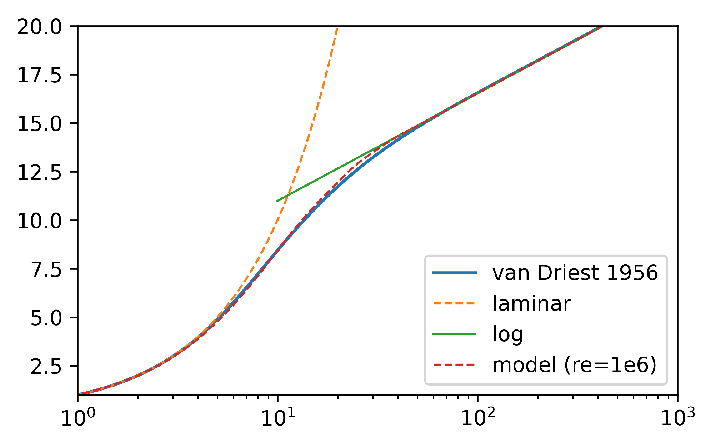
\includegraphics[width=0.66\textwidth]{Fig11.eps}} %vanDriest_profile.eps}}
  \caption{Near-wall velocity profile according to the 
    van-Driest scaling (blue, solid) in comparison with 
    the present model (red, dashed), 
    the viscous law of the wall (orange dashed), and 
    the logarithmic law (green, solid)} 
  \label{fig:vanDriest}
\end{figure}  An alternative approach that considers viscous effects close to the surface is the van-Driest scaling \citep{vandriest:JOT1956}, 
where an exponential damping of Prandtl's mixing length is considered near the wall to yield 
\begin{align}
  \frac{\p u^+}{\p z^+} = \frac{2}{ 1+ \sqrt{1+\left(2\kappa z^+\right)^2 (1-\exp\left[-z^+\right])}};
\end{align}
the spanwise component is zero as no rotational effects are considered. 
%
Comparing our proposed formulation for the stream-wise velocity in the inner layer to  \citeauthor{vandriest:JOT1956}'s formulation yields later convergence of the velocity onto the logarithmic profile while, over all, it serves as an excellent model of the streamwise velocity component (Fig.~\ref{fig:vanDriest}):
% 
Notable deviations (on the order of few percent) only occur in the region $10 < z^+ < 30$,  where the velocity transitions from the linear to the logarithmic profile. 
%
\par
%
%EKMAN SPIRAL 
For the higher layers of the ABL, the Ekman spiral is the simplest model available. 
%
When employed across the entirety of the ABL, the spiral of a turbulent Ekman layer is flattened with respect to Ekman's laminar solution, which  corresponds to a reduction of the veering angle both at the surface and throughout the ABL. 
%
We, however, find that a modified version of the Ekman spiral explicitly taking into account the surface boundary condition, is a consistent model and yields excellent agreement with the velocity profiles from DNS (Sec.~\ref{sec:ekman}). 

%ETLING MODEL 
\begin{figure}
  \textbf{(a)\hspace{0.48\textwidth}(b)}\\[-0.15em]
  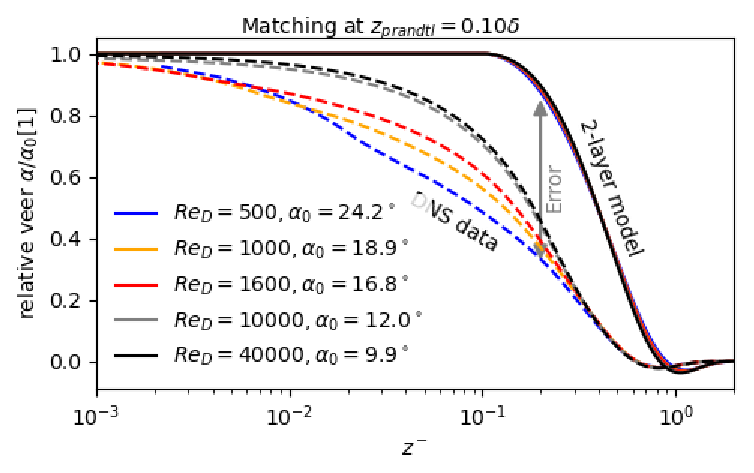
\includegraphics[width=0.5\textwidth]{Fig12a.eps} %etling_direction.eps} 
  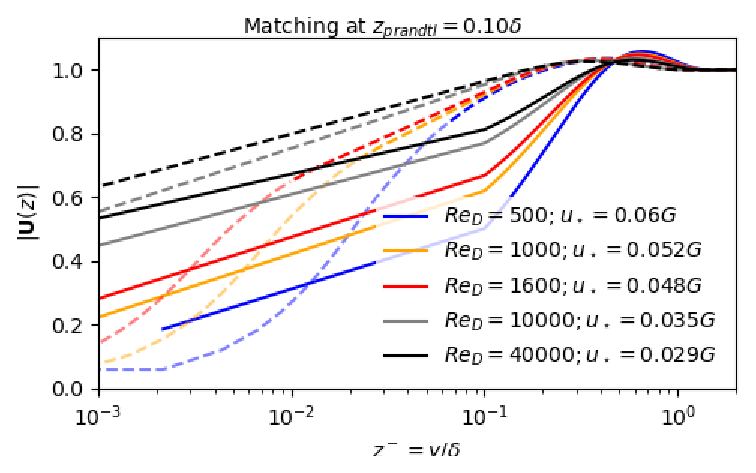
\includegraphics[width=0.5\textwidth]{Fig12b.eps} %etling_magnitude.eps}
  \caption{Comparison of the DNS data (dashed lines) with the two-layer model proposed by Etling (solid lines) for different Reynolds number. Left panel shows the relative wind veer, right panel shows the velocity magnitude. The Etling model is calibrated by the surface veer from the DNS and the roughness parameter is chosen according to the correction factor $\exp{\kappa A}$ such that the total veer and velocity magnitude agree. Profiles in the buffer layer, defined here as $z^+<30$ are shown as opaque dashed lines as the two-layer model does not consider viscous effects.}
  \label{fig:etling} 
\end{figure}
A two-layer model consolidating both the logarithmic and Ekman layer can be obtained following the arguments by \cite{etling:2008}, cf. \cite{emeis:2018}. Given a surface veering and a matching height (extent of the logarithmic layer), a formulation for the velocity profile across both the logarithmic and the outer layer is obtained. A comparison using the surface veering based on our model and a matching height of $z_\text{prandtl}=0.05\delta$, which gives better results than the matching height of $0.1\delta$ suggested by \cite{etling:2008}, is shown in Fig.~\ref{fig:etling}. 
% 
The overall shape of velocity magnitude is matched apart from the viscous and buffer layer (cf. Fig.~\ref{fig:etling}b) that is neglected by the two-layer model. However, quantitative departures on the order of 10\% occur across the inner layer: it turns out that the non-rotating profile, of the two-layer model in the logarithmic region yields too low overall velocity as the spanwise component contributes to the velocity across the inner layer. 
% 
Deviations also occur with respect to wind direction; despite the rather low matching height, a substantial fraction of the rotation occurs within the lower part of the ABL and about 20\% of the wind veer is not captured by the two-layer model. 
% 
As the overall veer is given, the non-captured veer close to the surface is then compensated across the logarithmic layer. In the upper part of the boundary layer, both profiles match well. 
% 
\par
% 
The interpretation of flux and gradient profiles in terms of the K-theory (cf. Sec.~\ref{sec:scaling}, Fig.~\ref{fig:stresses}) suggests a certain universality in the inner layer, while a global collapse, i.e. across the boundary layer, is not 
obtained. 
% 
While the K-Profiles concern the total stress, a consistent formulation of the turning would also require its partitioning to the individual components, i.e. the orientation of the stress vector $(\overline{u'w'}, \overline{v'w'})$ in the horizontal plane. If K-theory shall be used, this stress vector needs to be anti-parallel to the corresponding stress vector $(\partial_z U, \partial_z V)$. 
% 
Fig.~\ref{fig:alignment} shows the direction of the velocity, gradient and stress  vectors across the boundary layer. It turns out that the negative stress vector with respect to the wind direction and the flux vectors (absolute) have an approximately similar direction. 
%
It appears that both rotate by about $270^\circ$ ($3\pi/2$) across the boundary layer. 
%
Apart from the lower part of the Ekman layer ($0.2<z^-<0.7$), where there is a slight dependence on $Re$, the direction of stress appears to be universal, which is a consequence of the Ekman profile introduced in Sec.~\ref{sec:ekman}. 
%
However, this implies a misalignment between the flux and the stress on the order of the wind turning, and indeed Fig.~\ref{fig:alignment}b shows a misalignment up to $\pi/8$. This is in accordance with the expectation by \cite[][Chap.~7.18]{Townsend:1976} and prevents the transfer of energy from the mean flow to turbulence at these heights, thus preventing a boundary-layer growth. 
% 
While the behavior in the inner layer seems to depend on $Re$, there emerges universality in the misalignment across the outer layer, suggesting that a consideration of misalignment in the context of K-theory is possible when developing formulations for higher-order quantities. 
%
\begin{figure}
  \textbf{(a)\hspace{0.48\textwidth}(b)}\\[-0.15em]
  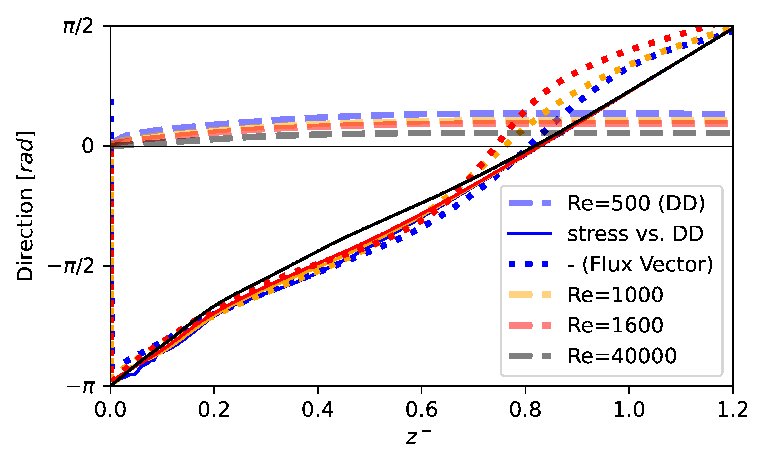
\includegraphics[width=0.5\textwidth]{Fig13a.eps} %stress_rotation.eps}
  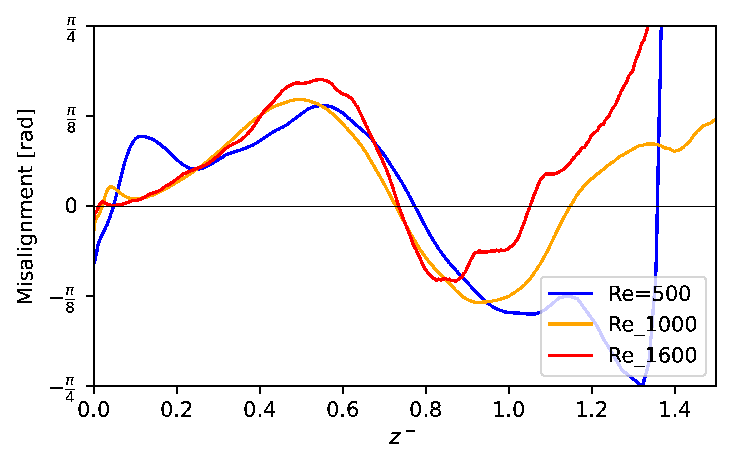
\includegraphics[width=0.5\textwidth]{Fig13b.eps} %misalignment.eps} 
  \caption{Panel \textbf{(a)} shows the wind direction (DD) as thick dashed lines and the direction of stress relative to DD as thin solid lines, both according to our profile model. The direction of the negative flux vector $(\overline{u'w'},\overline{v'w'})$ based on DNS data is shown as a dotted line. In panel \textbf{(b)}, we plot the misalignment, i.e. the angle, between the flux vector and the shear vector, where the shear vector is defined accordingly as $(\p_z U, \p_z V)$.} 
  \label{fig:alignment}
\end{figure}


% \textbf{Compare} Gryning (2007); highlight explicit knowledge on veering-profile % $\rightarrow$ directional sheer;
%% \textbf{Remember} of interpretation in the context of eddy viscosity (Fig.~\ref{fig:stresses}) 
% Consider Townsend ``Turbulent Shear Flow''  Chapter 7.18: p. 319 
% Implications for \textbf{K-theory} (we now can consider that shear and stress are not necessarily perfectly aligned).
% $\rightarrow$ can we do something to infer a K-profile from these theoretical considerations? 
%
\par%%%%%%%%%%%%%%%%%%%%%%%%%%%%%%%%%%%%%%%%%%%%%%%%%%%%%%%%%%%%%%%%%%%%%%%%%%%%%%%%
%

%
%\begin{figure}
%  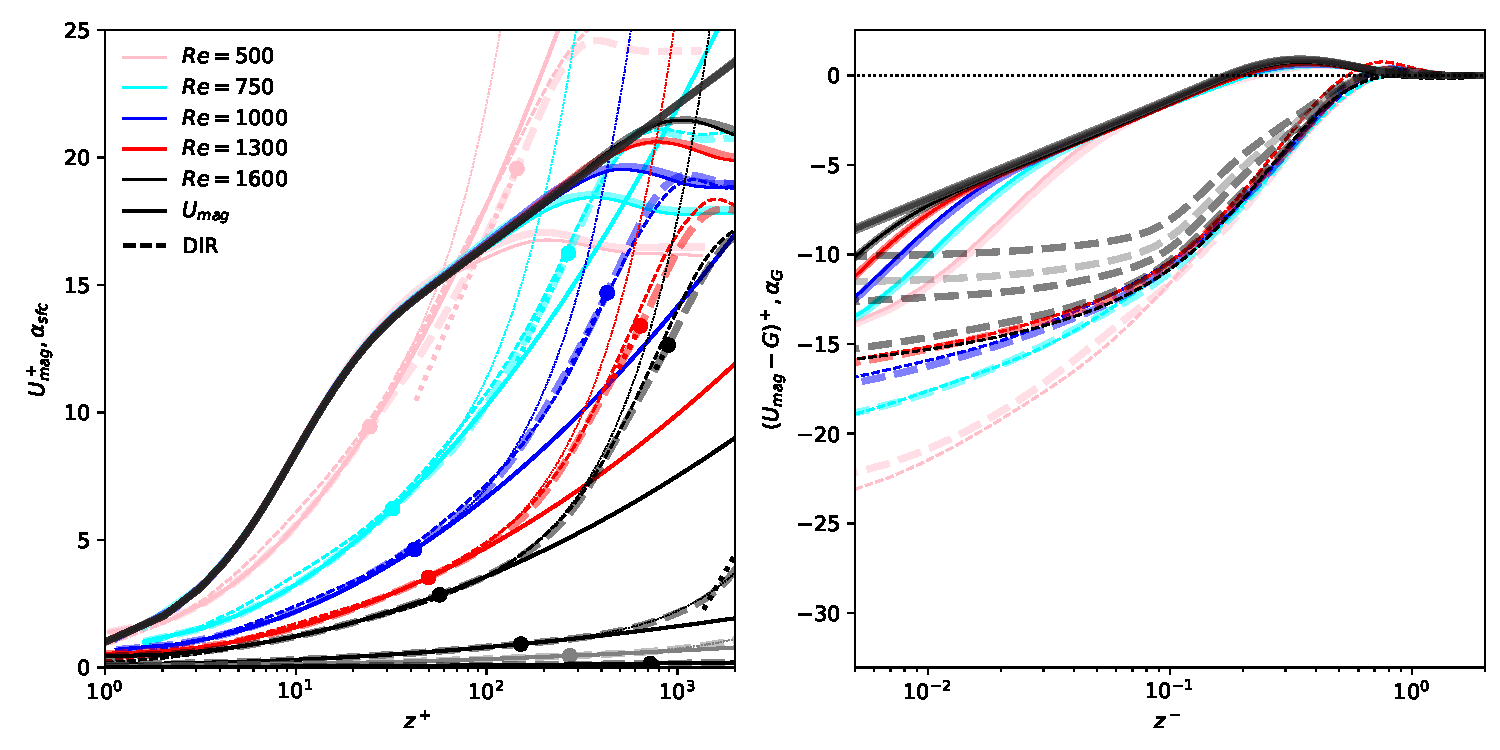
\includegraphics[width=\textwidth]{mag_dir.eps} 
%  \caption{Total velocity and veering (in degrees) vs inner and outer height.
%    Dashed lines show DNS data, thick lines are from semi-empirical theory.} 
%\end{figure} 
%
\section{Conclusions}
%
We investigate the wind veer and fundamental scaling properties of the velocity profiles in Ekman flow. 
%
Based on scaling considerations and direct numerical simulation spanning on decade in external separation from $Re_\Lambda=1.25 \times 10^5$ to $Re_\Lambda=1.28\times 10^6$, we derive a closed formulation for both horizontal components of the velocity profile in a stationary, smooth Ekman layer.  
% 
This formulation is consistent with the DNS data and also yields reasonable results  at geophysical scale separation; the logarithmic law of the mean velocity is recovered with the well-known limits and deviations towards the surface and Ekman layer. 
%
The classic formulation of the Ekman layer, employing the surface boundary condition, is replaced by a modified solution that can be obtained by Ekman's system of governing equations, but using different boundary conditions that are more appropriate of the actual situation encountered in the planetary boundary layer. 
% 
The three parameters that characterize this boundary condition are estimated based on DNS data. 
% 
\par
% 
To quantify the spanwise velocity component consistently across the boundary layer, we derive a universal scaling of the spanwise velocity component in a shear-aligned reference frame. For the \emph{inner layer}, we find the mixed scaling  
%
\begin{equation} 
  V^{\alpha_\star}/G = \frac{1}{\delta^+} f(z^+)
\end{equation}
%
that is, the spanwise velocity normalized by the outer velocity scale is a universal function of the inner height and Friction Reynolds number $Re_\tau = \delta^+$. 
% 
This scaling is derived here based on scaling considerations, and it is in excellent agreement with the DNS data available.   
% 
In the outer layer, the spanwise velocity follows outer scaling, consistently with the Ekman model discussed above (Sec.~\ref{sec:ekman}).
% 
\par
% 
Our results suggest that there is no lower limit of the turning. 
% 
Hence---despite its very large scale separation / huge Reynolds number---the ABL is not 
in the 'limit' of high Reynolds number from the perspective of wind veer, but always in a regime where 
changes in $\RE$ impact on the vertical partitioning of rotation. 



%\subsection{Applications \& Outlook} 
%\begin{itemize}
%\item reference-shear for neutral profile approaches(systematic!) $\rightarrow$ wind engineering! 
%\item initial condition for LES/DNS to eliminate/minimize inertial oscillation in Benchmark simulations
%\item
%\end{itemize} 


\appendix
\section{Appendices}
\subsection{Laminar Ekman solution with consideration of inner layer}
\label{app:ekman_solution}
The following Ekman system is obtained by averaging the Navier--Stokes equations horizontally and over time and neglecting the turbulent transport terms (turbulence can then be considered via variation of the vertically constant eddy viscosity $\nu$; for a height-dependent eddy-viscosity model, the reader is referred to \cite{basu:BM2023}):
\begin{subequations}
\begin{eqnarray}
  \left(\begin{matrix}
    \p_t U\\
    \p_t V  
  \end{matrix}\right)&=&\left(\begin{matrix}
     fV &+& \nu \p_z^2 U\\ 
    -f(U-G) &+& \nu \p_z^2 V
  \end{matrix}\right)\\ 
  \Rightarrow \partial_t (U+iV) &=& f(V-i(U-G))) + \nu \p_z^2(U+iV)
\end{eqnarray}
In stationary conditions, this system is solved by
\begin{eqnarray}
  \hat{u}(z) &=& U_{\infty} + e^{-\gamma z} \left[A \cos\gamma z + B \sin\gamma z\right]   \\
  \hat{v}(z) &=& V_{\infty} + e^{-\gamma z} \left[-A \sin\gamma z + B \cos\gamma z\right]
\end{eqnarray} 
\end{subequations}
where the constants $U_\infty$, $V_\infty$ set the top boundary condition and $A$ and $B$ set the bottom boundary condition. 
%
The most common boundary condition for a surface Ekman layer is $A=U_{\infty}=G$, $B=0$, and $V_{\infty}=0$.
%
The lower boundary condition, however, neglects the existence of the surface layer, and it appears reasonable to define
$A=c G$ where $c<1$ is a constant that incorporates the increased shear in the surface layer.
%
Given a 'matching height' $z_{match}$ and normalized matching height $\xi=\gamma z_\text{match}$ in the upper part of the inner layer, we can match the Ekman profile
to the inner layer by letting
%
\begin{subequations}
\begin{eqnarray}
  \begin{matrix} 
    u(z_\text{match}) \equiv u_\text{match} &=& U_{\infty} + e^{-\gzm} \left [ A \cos\gzm + B\sin\gzm \right] \\
    v(z_\text{match}) \equiv v_\text{match} &=& V_{\infty} + e^{-\gzm} \left [-A \sin\gzm + B\cos\gzm \right]
  \end{matrix} 
\end{eqnarray}
\begin{eqnarray}
  \Rightarrow \left(\begin{matrix}
    u_\text{match}-U_{\infty} \\ 
    v_\text{match}-V_{\infty}
  \end{matrix}\right) = e^{-\gzm}\left(\begin{matrix}A \\ B \end{matrix}\right)\left(\begin{matrix}
    \cos\gzm &+ \sin\gzm \\ -\sin\gzm &+ \cos\gzm
  \end{matrix} \right) \\
\end{eqnarray}
\end{subequations}
Matching the profile at $\xi=0$, one obtains
$A = \Delta u_\text{match} $ and $B=-\Delta w_\text{match} $; and when the direction $Ox$ is aligned
with the geostrophic wind, we obtain the textbook-case $A=|\mathbf{G}|$ and $B=0$. 

Otherwise, choosing $B \ne 0$ allows to introduce a phase shift of the Ekman rotation with respect to
the decay of the wind spiral.
%
However, in our context, the thickness and position of the spiral can already be controlled by
the eddy viscosity and an offset in $\xi$, here we let $B=0$.
%%%%%%%%%%%%%%%%%%%%%%%%%%%%%%%%%%%%%%%%%%%%%%%%%%%%%%%%%%%%%%%%%%%%%%%%%%%%%%%%
%% Determining parameters A and B from profile values at a given height
%%%%%%%%%%%%%%%%%%%%%%%%%%%%%%%%%%%%%%%%%%%%%%%%%%%%%%%%%%%%%%%%%%%%%%%%%%%%%%%%
%% 
%% \begin{subequations} 
%% \begin{eqnarray}
%%   e^\gzm \Delta u_\text{match} = A \cos\gzm + B\sin\gzm \\
%%   e^\gzm (\cos\gzm \Delta u_\text{match} - \sin\gzm \Delta w_\text{match}) = A (\cos^2\gzm + \sin^2\gzm)
%% \end{eqnarray}
%% \begin{eqnarray}
%%   \Rightarrow A &=&e^\gzm (\cos\gzm\Delta u_\text{match} + \sin\gzm \Delta w_\text{match})\\
%%   B&=&  \frac{e^\gzm \Delta u_\text{match} - A \cos \gzm}{\sin\gzm} \\
%%   &=& e^\gzm \frac{ \sin^2\gzm \Delta u_\text{match}+\sin\xi\cos\xi \Delta w_\text{match} }{\sin\xi }  \\
%%   &=& e^\gzm (\sin\xi\Delta u_\text{match} + \cos\xi\Delta w_\text{match}) 
%% \end{eqnarray}
%% \end{subequations} 

\subsection{Matching the spanwise velocity profiles in the inner layer}

\label{app:log-coefficients}
The spanwise profile in vicinity of the surface is given by
$V/G=f_{V,\mathrm{visc}}\delta ^+$ with
\begin{subequations}
\begin{eqnarray}
  f_{V,\mathrm{visc}} &=& v_\mathrm{ref}\left(\omega_v z^+ -1 + e^{-\omega_v z^+}\right)\\
  f_{V,\mathrm{log}}   &=& a_\mathrm{log} + b_\mathrm{log} \log z^+ + c_\mathrm{log} z^+ 
\end{eqnarray}
\end{subequations}
Matching the profiles and gradient $z_0=10^+$ and the value at $z_1=0.3\delta^+$ yields
\begin{subequations} 
\begin{eqnarray}
  v_\mathrm{ref} \left(\omega_v z_{0} + e^{-\omega_v z_{0}}\right)
  & = v_{0}=& a_\mathrm{log} + b_\mathrm{log} \log z_{0} +c_\mathrm{log} z_{0}  \\
  &   v_{1}=& a_\mathrm{log} + b_\mathrm{log} \log z_{1} +c_\mathrm{log} z_{1} \\
  v_\mathrm{ref}\omega_z \left( 1 - e^{-\omega_z z_{0}}\right)
  & = d_{0}=& \frac{b_\mathrm{log}}{z_{10}} + c_\mathrm{log} 
\end{eqnarray}
\end{subequations} 
The gradient condition implies $b_\mathrm{log}=(d_{0} -c_\mathrm{log})z_{0}$, and yields
\begin{subequations}
\begin{eqnarray}
  %v_{0}&=& a_\mathrm{log} + z_{0}\left[ (d_0-c_\mathrm{log}) \log z_{0} +c_\mathrm{log}\right]\\
  v_0-z_0d_0\log z_0&=& a_\mathrm{log} + c_\mathrm{log} (z_0- z_0\log z_0) \\
  %v_1 &=& a_\mathrm{log} + z_0(d_0-c_\mathrm{log})\log z_1 +  c_\mathrm{log}z_1\\ 
  v_1-z_0d_0\log z_1 &=& a_\mathrm{log} +c_\mathrm{log} (z_1- z_0\log z_0)  \\
  \Rightarrow c_\mathrm{log}&=& \frac{ \Delta v - z_0d_0 \log z_1/z_0}{\Delta z} 
\end{eqnarray}
with $\Delta z=z_1-z_0$ and $\Delta v=v_1-v_0$.
%
Then, the coefficient $a_\mathrm{log}$ is estimated as 
\begin{eqnarray} 
  a_\mathrm{log} &=& v_0-z_0d_0\log z_0 -  \frac{ \Delta v - z_0d_0 \log z_1/z_0}{\Delta z}\left[
    z_0-z_0\log z_0 
    \right]. 
\end{eqnarray}
We note that $ \log(z_1/z_0) / (z_1-z_0) \rightarrow 0$ for large $z_1$, and as $z_1=0.3\delta^+$,
this implies that the second term in $c_\mathrm{log}$ only plays a role at low and intermediate $\RE$.
Then, $a_\mathrm{log}$ can be estimated as 
\begin{eqnarray}
  a_\mathrm{log} \simeq v_0 -z_0 \left[ d_0 \log  z_0 - \frac{\Delta v}{\Delta z} ( 1- \log z_0) \right] 
\end{eqnarray}
for large $\RE$. 
\end{subequations}


\vspace{1em}
\noindent\textbf{Acknowledgements} We thank Sukanta Basu and two anonymous reviewers for their valuable reviews of this manuscript. Simulations were carried out on the German supercomputing systems 
\texttt{hawk} at H\"ocstleistungsrechenzentrum Stuttgart (Bundesprojekt 44187) and \texttt{juwels} at Gauss Centre for supercomputing, 
For\-schungs\-zen\-trum J\"ulich (Projects \texttt{hku24} and \texttt{stadit}). 
We extend our thanks to Sally Issa for valuable feedback on the manuscript. 



\section*{Declarations} 

\noindent\textbf{Author contributions} CA conceived the study, acquired funding, performed the simulation, analysed and plotted the data for this work. CA and HW interpreted the data and compiled the manuscript. 
\vspace{1em} 

\noindent\textbf{Funding} CA is funded by the European Commission's 7$^{th}$ Framework Programme through 
the ERC 2019 Starting Grant trainABL (ID 851374). HW is funded by the Ministry for Science and Culture of 
Lower Saxony (project \emph{Zukunftskonzept Windenergieforschung}). Open Access funding for this publication through the DEAL agreement. 
\vspace{1em}

\noindent\textbf{Data availability} The data is available in long-term repositories and indexed by DOIs as cited in the list of references. Further analysis tools and processed data can be made available upon direct request. \vspace{1em}

\noindent\textbf{Conflict of interest} The Authors declare no competing interest.
\vspace{1em}

\noindent\textbf{Open access} This article is licensed under a Creative Commons Attribution 4.0 International License, which permits use, sharing, adaptation, distribution and reproduction in any medium or format, as long as you give appropriate credit to the original author(s) and the source, provide a link to the Creative Commons licence, and indicate if changes were made.  To view a copy of this licence, visit \href{http://creativecommons.org/licenses/by/4.0/}{https://creativecommons.org/licenses/by/4.0/}.


\bibliographystyle{spbasic_updated}  
% \bibliography{ansorge}
\begin{thebibliography}{57}
\providecommand{\natexlab}[1]{#1}
\providecommand{\url}[1]{{#1}}
\providecommand{\urlprefix}{URL }
\expandafter\ifx\csname urlstyle\endcsname\relax
  \providecommand{\doi}[1]{DOI~\discretionary{}{}{}#1}\else
  \providecommand{\doi}{DOI~\discretionary{}{}{}\begingroup
  \urlstyle{rm}\Url}\fi
\providecommand{\eprint}[2][]{\url{#2}}

\bibitem[{Ansorge(2019)}]{ansorge:BM2019}
Ansorge C (2019) Scale {{Dependence}} of {{Atmosphere}}--{{Surface Coupling
  Through Similarity Theory}}. Boundary-Layer Meteorol 170(1):1--27,
  \doi{10.1007/s10546-018-0386-y}

\bibitem[{Ansorge(2024{\natexlab{a}})}]{ansorge:2024c}
Ansorge C (2024{\natexlab{a}}) Direct numerical simulation of turbulent
  {{Ekman}} flow ({{Re}}=0500): {{DOI}} 10.17169/refubium-42505.
  \doi{10.17169/refubium-42505}

\bibitem[{Ansorge(2024{\natexlab{b}})}]{ansorge:2024a}
Ansorge C (2024{\natexlab{b}}) Direct numerical simulation of turbulent
  {{Ekman}} flow ({{Re}}=1000): {{DOI}} 10.17169/refubium-42507.
  \doi{10.17169/refubium-42507}

\bibitem[{Ansorge(2024{\natexlab{c}})}]{ansorge:2024}
Ansorge C (2024{\natexlab{c}}) Direct numerical simulation of turbulent
  {{Ekman}} flow ({{Re}}=1300): {{DOI}} 10.17169/refubium-42508.
  \doi{10.17169/refubium-42508}

\bibitem[{Ansorge(2024{\natexlab{d}})}]{ansorge:2024b}
Ansorge C (2024{\natexlab{d}}) Direct numerical simulation of turbulent
  {{Ekman}} flow ({{Re}}=1600); {{DOI}} 10.17169/refubium-42509.
  \doi{10.17169/refubium-42509}

\bibitem[{Ansorge and Mellado(2014)}]{ansorge:BM2014}
Ansorge C, Mellado JP (2014) Global {{Intermittency}} and {{Collapsing
  Turbulence}} in the {{Stratified Planetary Boundary Layer}}. Boundary-Layer
  Meteorol 153(1):89--116, \doi{10.1007/s10546-014-9941-3}

\bibitem[{Ansorge and Mellado(2016)}]{ansorge:JFM2016}
Ansorge C, Mellado JP (2016) Analyses of external and global intermittency in
  the logarithmic layer of {{Ekman}} flow. J Fluid Mech 805:611--635,
  \doi{10.1017/jfm.2016.534}

\bibitem[{Baars and Marusic(2020)}]{baars:JFM2020a}
Baars WJ, Marusic I (2020) Data-driven decomposition of the streamwise
  turbulence kinetic energy in boundary layers. {{Part}} 2. {{Integrated}}
  energy and. J Fluid Mech 882:A26, \doi{10.1017/jfm.2019.835}

\bibitem[{Barenblatt(1993)}]{barenblatt:JFM1993}
Barenblatt GI (1993) Scaling laws for fully developed turbulent shear flows.
  {{Part}} 1. {{Basic}} hypotheses and analysis. J Fluid Mech 248:513--520,
  \doi{10.1017/S0022112093000874}

\bibitem[{Barenblatt and Goldenfeld(1995)}]{barenblatt:PF1995}
Barenblatt GI, Goldenfeld N (1995) Does fully developed turbulence exist?
  {{Reynolds}} number independence versus asymptotic covariance. Phys Fluids
  7(12):3078--3082, \doi{10/bw2sqs}

\bibitem[{Basu and Holtslag(2023)}]{basu:BM2023}
Basu S, Holtslag AAM (2023) A novel approach for deriving the stable boundary layer height and eddy viscosity concepts from the Ekman equations. Boundary-Layer Meteorol (187):105--115, \doi{}

\bibitem[{Blackadar and Tennekes(1968)}]{blackadar:JAS1968}
Blackadar AK, Tennekes H (1968) Asymptotic {{Similarity}} in {{Neutral
  Barotropic Planetary Boundary Layers}}. Journal of the Atmospheric Sciences
  25:1015--1020, \doi{10.1175/1520-0469(1968)025<1015:ASINBP>2.0.CO;2}

\bibitem[{Brown et~al.(2005)Brown, Beljaars, Hersbach, Hollingsworth, Miller,
  and Vasiljevic}]{brown:QJR2005}
Brown AR, Beljaars ACM, Hersbach H, Hollingsworth A, Miller M, Vasiljevic D
  (2005) Wind turning across the marine atmospheric boundary layer. Quarterly
  Journal of the Royal Meteorological Society 131(607):1233--1250,
  \doi{10/dw2bxz}

\bibitem[{Calaf et~al.(2010)Calaf, Meneveau, and Meyers}]{calaf:PF2010}
Calaf M, Meneveau C, Meyers J (2010) Large eddy simulation study of fully
  developed wind-turbine array boundary layers. Phys Fluids 22(1):015,110,
  \doi{10/b7gc6v}

\bibitem[{Coleman et~al.(1992)Coleman, Ferziger, and Spalart}]{coleman:JFM1992}
Coleman GN, Ferziger JH, Spalart PR (1992) Direct {{Simulation}} of the
  {{Stably Stratified Turbulent Ekman Layer}}. Journal of Fluid Mechanics
  244:677--712, \doi{10.1017/S0022112092003264}

\bibitem[{{da Silva} et~al.(2014){da Silva}, Hunt, Eames, and
  Westerweel}]{dasilva:ARF2014}
{da Silva} CB, Hunt JC, Eames I, Westerweel J (2014) Interfacial {{Layers
  Between Regions}} of {{Different Turbulence Intensity}}. Annu Rev Fluid Mech
  46(1):567--590, \doi{10.1146/annurev-fluid-010313-141357}

\bibitem[{Dimotakis(2005)}]{dimotakis:ARF2005}
Dimotakis PE (2005) {{TURBULENT MIXING}}. Annual Review of Fluid Mechanics
  37(1):329--356, \doi{10.1146/annurev.fluid.36.050802.122015}

\bibitem[{Ekman(1905)}]{ekman:AMA1905}
Ekman VW (1905) On the influence of the earth's rotation on ocean currents. Ark
  Mat Astron Fys, Vol 2 (1905), pp 1-53 2:1--53

\bibitem[{Ellison(1955)}]{ellison:QJR1955}
Ellison TH (1955) The {{Ekman}} spiral. Q J Roy Met Soc 81(350):637--638,
  \doi{10.1002/qj.49708135025}

\bibitem[{Emeis(2018)}]{emeis:2018}
Emeis S (2018) Wind {{Energy Meteorology}}, 2nd edn. Atmospheric {{Physics}}
  for {{Wind Power Generation}}, Springer, Heidelberg

\bibitem[{Emeis et~al.(2007)Emeis, {Baumann-Stanzer}, Piringer, Kallistratova,
  Kouznetsov, and Yushkov}]{emeis:m2007}
Emeis S, {Baumann-Stanzer} K, Piringer M, Kallistratova M, Kouznetsov R,
  Yushkov V (2007) Wind and turbulence in the urban boundary layer analysis
  from acoustic remote sensing data and fit to analytical relations. metz
  16(4):393--406, \doi{10.1127/0941-2948/2007/0217}

\bibitem[{Esau(2004)}]{esau:EFM2004}
Esau I (2004) Simulation of {{Ekman Boundary Layers}} by {{Large Eddy Model}}
  with {{Dynamic Mixed Subfilter Closure}}. Environmental Fluid Mechanics
  4(3):273--303, \doi{10/b8f3kh}

\bibitem[{Etling(2002)}]{etling:2002}
Etling D (2002) Theoretische {{Meteorologie}}, 2nd edn. Eine
  {{Einf{\"u}hrung}}, Springer-Verlag, Berlin, Heidelberg

\bibitem[{Etling(2008)}]{etling:2008}
Etling D (2008) {Theoretische Meteorologie: eine Einf{\"u}hrung}, 3rd edn.
  Springer, Berlin Heidelberg

\bibitem[{Foken(2002)}]{foken:m2002}
Foken T (2002) Some aspects of the viscous sublayer. metz 11(4):267--272,
  \doi{10.1127/0941-2948/2002/0011-0267}

\bibitem[{Foken et~al.(1978)Foken, Kitajgorodskij, and Kuznecov}]{foken:BM1978}
Foken {\relax Th}, Kitajgorodskij SA, Kuznecov OA (1978) On the dynamics of the
  molecular temperature boundary layer above the sea. Boundary-Layer Meteorol
  15(3):289--300, \doi{10.1007/BF02652602}

\bibitem[{Ghannam and {Bou-Zeid}(2021)}]{ghannam:QJR2021}
Ghannam K, {Bou-Zeid} E (2021) Baroclinicity and directional shear explain
  departures from the logarithmic wind profile. Quarterly Journal of the Royal
  Meteorological Society 147:434--464, \doi{10/gnj6z2}

\bibitem[{Gryning et~al.(2007)Gryning, Batchvarova, Br{\"u}mmer, J{\o}rgensen,
  and Larsen}]{gryning:BM2007}
Gryning SE, Batchvarova E, Br{\"u}mmer B, J{\o}rgensen H, Larsen S (2007) On
  the extension of the wind profile over homogeneous terrain beyond the surface
  boundary layer. Boundary-Layer Meteorol 124(2):251--268,
  \doi{10.1007/s10546-007-9166-9}

\bibitem[{H{\"o}gstr{\"o}m(1988)}]{hogstrom:BM1988}
H{\"o}gstr{\"o}m U (1988) Non-dimensional wind and temperature profiles in the
  atmospheric surface layer: {{A}} re-evaluation. Boundary-Layer Meteorology
  42:55--78, \doi{10.1007/BF00119875}

\bibitem[{H{\"o}gstr{\"o}m(1996)}]{hogstrom:BM1996}
H{\"o}gstr{\"o}m U (1996) Review of some basic characteristics of the
  atmospheric surface layer. Boundary-Layer Meteorology 78(3-4):215--246,
  \doi{10.1007/BF00120937}

\bibitem[{Jacobs and Van~Boxel(1988)}]{jacobs:AFM1988}
Jacobs AF, Van~Boxel JH (1988) Changes of the displacement height and roughness
  length of maize during a growing season. Agricultural Forest Meteorol
  42(1):53--62, \doi{10.1016/0168-1923(88)90066-4}

\bibitem[{Jiang et~al.(2018)Jiang, Wang, and Sullivan}]{jiang:JAS2018}
Jiang Q, Wang S, Sullivan P (2018) Large-{{Eddy Simulation Study}} of {{Log
  Laws}} in a {{Neutral Ekman Boundary Layer}}. Journal of the Atmospheric
  Sciences 75(6):1873--1889, \doi{10.1175/JAS-D-17-0153.1}

\bibitem[{Jim{\'e}nez(2012)}]{jimenez:ARF2012}
Jim{\'e}nez J (2012) Cascades in {{Wall-Bounded Turbulence}}. Ann Rev Fluid
  Mech 44(Volume 44, 2012):27--45, \doi{10.1146/annurev-fluid-120710-101039}

\bibitem[{Kelly and Gryning(2010)}]{kelly:BM2010}
Kelly M, Gryning SE (2010) Long-{{Term Mean Wind Profiles Based}} on
  {{Similarity Theory}}. Boundary-Layer Meteorol 136(3):377--390,
  \doi{10.1007/s10546-010-9509-9}

\bibitem[{Kelly and Troen(2016)}]{kelly:WE2016}
Kelly M, Troen I (2016) Probabilistic stability and `tall' wind profiles:
  Theory and method for use in wind resource assessment. Wind Energy
  19(2):227--241, \doi{10.1002/we.1829}

\bibitem[{Klein et~al.(2021)Klein, Maier, and Schmidt}]{klein:PAM2021a}
Klein M, Maier RE, Schmidt H (2021) Stochastic modeling of transient neutral
  and stably-stratified {{Ekman}} boundary layers. P A M M 21(1):e202100,146,
  \doi{10.1002/pamm.202100146}

\bibitem[{Li et~al.(2018)Li, Gentine, Mellado, and McColl}]{li:JAS2018}
Li Q, Gentine P, Mellado JP, McColl KA (2018) Implications of {{Nonlocal
  Transport}} and {{Conditionally Averaged Statistics}} on {{Monin}}--{{Obukhov
  Similarity Theory}} and {{Townsend}}'s {{Attached Eddy Hypothesis}}. J Atmos
  Sci 75(10):3403--3431, \doi{10.1175/JAS-D-17-0301.1}

\bibitem[{Lindvall and Svensson(2019)}]{lindvall:QJR2019}
Lindvall J, Svensson G (2019) Wind turning in the atmospheric boundary layer
  over land. Q J Roy Met Soc 145(724):3074--3088, \doi{10.1002/qj.3605}

\bibitem[{Mellado and Ansorge(2012)}]{mellado:ZaM2012}
Mellado J, Ansorge C (2012) Factorization of the {{Fourier}} transform of the
  pressure-{{Poisson}} equation using finite differences in colocated grids. Z
  angew Math Mech 92(5):380--392, \doi{10.1002/zamm.201100078}

\bibitem[{Mellado et~al.(2016)Mellado, {van Heerwaarden}, and
  Garcia}]{mellado:BM2016}
Mellado JP, {van Heerwaarden} CC, Garcia JR (2016) Near-{{Surface Effects}} of
  {{Free Atmosphere Stratification}} in {{Free Convection}}. Boundary-Layer
  Meteorol 159(1):69--95, \doi{10.1007/s10546-015-0105-x}

\bibitem[{Mirocha et~al.(2018)Mirocha, Churchfield, {Mu{\~n}oz-Esparza}, Rai,
  Feng, Kosovi{\'c}, Haupt, Brown, Ennis, Draxl, Sanz~Rodrigo, Shaw, Berg,
  Moriarty, Linn, Kotamarthi, Balakrishnan, Cline, Robinson, and
  Ananthan}]{mirocha:WES2018}
Mirocha JD, Churchfield MJ, {Mu{\~n}oz-Esparza} D, Rai RK, Feng Y, Kosovi{\'c}
  B, Haupt SE, Brown B, Ennis BL, Draxl C, Sanz~Rodrigo J, Shaw WJ, Berg LK,
  Moriarty PJ, Linn RR, Kotamarthi VR, Balakrishnan R, Cline JW, Robinson MC,
  Ananthan S (2018) Large-eddy simulation sensitivities to variations of
  configuration and forcing parameters in canonical boundary-layer flows for
  wind energy applications. Wind Energy Science 3(2):589--613, \doi{10/gn3nh4}

\bibitem[{Moin and Mahesh(1998)}]{moin:ARF1998}
Moin P, Mahesh K (1998) Direct numerical simulation: {{A}} tool in turbulence
  research. Annual Review of Fluid Mechanics 30:539--578,
  \doi{10.1146/annurev.fluid.30.1.539}

\bibitem[{Momen and {Bou-Zeid}(2016)}]{momen:JAS2016}
Momen M, {Bou-Zeid} E (2016) Large-{{Eddy Simulations}} and {{Damped-Oscillator
  Models}} of the {{Unsteady Ekman Boundary Layer}}*. Journal of the
  Atmospheric Sciences 73(1):25--40, \doi{10.1175/JAS-D-15-0038.1}

\bibitem[{Momen et~al.(2018)Momen, {Bou-Zeid}, Parlange, and
  Giometto}]{momen:JAS2018}
Momen M, {Bou-Zeid} E, Parlange MB, Giometto M (2018) Modulation of {{Mean
  Wind}} and {{Turbulence}} in the {{Atmospheric Boundary Layer}} by
  {{Baroclinicity}}. Journal of the Atmospheric Sciences 75(11):3797--3821,
  \doi{10/gfmn67}

\bibitem[{Monin(1970)}]{monin:ARF1970}
Monin AS (1970) The {{Atmospheric Boundary Layer}}. Annual Review of Fluid
  Mechanics 2:225--250, \doi{10.1146/annurev.fl.02.010170.001301}

\bibitem[{Monin and Yaglom(1975)}]{monin:1975}
Monin AS, Yaglom AM (1975) Statistical {{Fluid Mechanics}}, {{Vol}}. {{II}},
  Dover {{Publications}} on {{Physics}}, vol~II. Dover Publications, Inc.,
  Mineola

\bibitem[{Optis et~al.(2014)Optis, Monahan, and Bosveld}]{optis:BM2014}
Optis M, Monahan A, Bosveld FC (2014) Moving {{Beyond Monin-Obukhov Similarity
  Theory}} in {{Modelling Wind-Speed Profiles}} in the {{Lower Atmospheric
  Boundary Layer}} under {{Stable Stratification}}. Boundary-Layer Meteorology
  153(3):497--514, \doi{10.1007/s10546-014-9953-z}

\bibitem[{Rossby and Montgomery(1935)}]{rossby:PIP1935}
Rossby CG, Montgomery RB (1935) The layer of frictional influence in wind and
  ocean currents. Papers in Physical Oceanography and Meteorology III(3):1--101

\bibitem[{Sakagami et~al.(2020)Sakagami, Haas, and Passos}]{sakagami:BM2020}
Sakagami Y, Haas R, Passos JC (2020) Generalized {{Non-dimensional Wind}} and
  {{Temperature Gradients}} in the {{Surface Layer}}. Boundary-Layer Meteorol
  175(3):441--451, \doi{10.1007/s10546-020-00510-3}

\bibitem[{Spalart(1989)}]{spalart:JFM1989}
Spalart PR (1989) Theoretical and numerical study of a three-dimensional
  turbulent boundary layer. J Fluid Mech 205(-1):319,
  \doi{10.1017/S0022112089002053}

\bibitem[{Spalart et~al.(2008)Spalart, Coleman, and Johnstone}]{spalart:PF2008}
Spalart PR, Coleman GN, Johnstone R (2008) Direct numerical simulation of the
  {{Ekman}} layer: {{A}} step in {{Reynolds}} number, and cautious support for
  a log law with a shifted origin. Phys Fluids 20(10):101,507,
  \doi{10.1063/1.3005858}

\bibitem[{Spalart et~al.(2009)Spalart, Coleman, and Johnstone}]{spalart:PF2009}
Spalart PR, Coleman GN, Johnstone R (2009) Retraction: ``{{Direct}} numerical
  simulation of the {{Ekman}} layer: {{A}} step in {{Reynolds}} number, and
  cautious support for a log law with a shifted origin'' [{{Phys}}. {{Fluids}}
  20, 101507 (2008)]. Phys Fluids 21(10):109,901, \doi{10.1063/1.3247176}

\bibitem[{Stoll et~al.(2020)Stoll, Gibbs, Salesky, Anderson, and
  Calaf}]{stoll:BM2020}
Stoll R, Gibbs JA, Salesky ST, Anderson W, Calaf M (2020) Large-{{Eddy
  Simulation}} of the {{Atmospheric Boundary Layer}}. Boundary-Layer Meteorol
  177(2-3):541--581, \doi{10/gmbmzw}

\bibitem[{Svensson and Holtslag(2009)}]{svensson:BM2009}
Svensson G, Holtslag AAM (2009) Analysis of {{Model Results}} for the
  {{Turning}} of the {{Wind}} and {{Related Momentum Fluxes}} in the {{Stable
  Boundary Layer}}. Boundary-Layer Meteorol 132(2):261--277, \doi{10/bwknmt}

\bibitem[{Tennekes(1973)}]{tennekes:JAS1973}
Tennekes H (1973) A {{Model}} for the {{Dynamics}} of the {{Inversion Above}} a
  {{Convective Boundary Layer}}. Journal of the Atmospheric Sciences

\bibitem[{Townsend(1976)}]{Townsend:1976}
Townsend AA (1976) The Structure of Turbulent Shear Flow, 2nd edn. Cambridge
  University Press

\bibitem[{Van~Driest(1956)}]{vandriest:JOT1956}
Van~Driest ER (1956) On {{Turbulent Flow Near}} a {{Wall}}. Journal of the
  Aeronautical Sciences 23(11):1007--1011, \doi{10.2514/8.3713}

\bibitem[{Zikanov et~al.(2003)Zikanov, Slinn, and Dhanak}]{zikanov:JFM2003}
Zikanov O, Slinn DN, Dhanak MR (2003) Large-eddy simulations of the
  wind-induced turbulent {{Ekman}} layer. J Fluid Mech 495:343--368,
  \doi{10/ccbpbw}

\end{thebibliography}



\end{document}
\appendix
\section{Old Stuff}
\todo{OLD FROM HERE} 
Below this region, the gradients in span-wise velocity are rather small and the span-wise velocity
monotonically approaches its surface boundary condition $V(z=0)=0$.
%
While the streamwise velocity follows a universal inner scaling that has acquired its universal, $Re$-independent shape for $Re_D> \mathcal{O}\left(10^3\right)$, the span-wise component that defines how the velocity vector veers when the surface is approached,
does not collapse in inner units, and there is, most importantly no sign of convergence even at the highest Reynolds numbers for
which simulations where carried out.
%
Even though the simplest assumption $V=0$ is reasonable for the lower part of the surface surface layer ($z^-<10^{-3}$), it does
not appropriately capture the profile in the rest of the surface layer:

First, $V=0$  implies a discontinuity in the velocity profile at $z^-=0.1$, where the outer scaling found above 
yields a finite value at geophysical $Re$, i.e. there is non-zero veering in the upper part of the
surface layer--as is well-known also from field observation. 
%
Second, the layer around $z^-=0.1$ is crucial to obtain the characteristic and well-established shape of the hodographs as the layer
where $V$ sets in marks the 'maximum' of $V^-$ vs. $U^-$.
%
%
\par
%
The scale for the magnitude of the span-wise velocity component is $u_\star\sin\alpha$. 
%
Based on our DNS data, we suggest that the Reynolds number scaling of this velocity-magnitude scale is captured
by $Re_\tau^{-1/2}$ which is indeed known from the generalization of higher-order statistics, such as turbulent fluxes
in the inner layer \citep{marusic:JFM2013} that also follow a mixed scaling in the inner layer.
%
We then parameterize the spanwise velocity at 10 wall units as anchor point in the inner layer:
\begin{subequations}
\begin{align}
  V_{10}\equiv V(z^+=10)=750 \frac{u_\star\sin\alpha}{\sqrt{Re_\tau}}.
\end{align} 
%
This leaves us with three fixed points of the velocity profile in the inner layer, namely
(i) the boundary condition $V_0=0$,
(ii) $V_{10}$ at $z^+=10$, and 
(iii) the lower end of the logarithmic profile at $z^-=0.1$ where the latter two are semi-empirically estimated
from DNS data. 
%
In absence of well-established scaling considerations for the span-wise velocity, the choice of profile fits joining
these three points is indeed arbitrary, but we can resort to the DNS data for an empirical approach and find
that a square-root profile fits $V(z^+)$ in the surface layer.
%
A linear profile for $V$ is employed in the viscous sub-layer.
%
Based on the physical extent of the viscous sub-layer in Ekman flow around five wall units \citep{foken:m2002, ansorge:BM2019},
we choose $z^+=5$ to transition from one to the other and note that $V$ is already very small at this height.
%
The span-wise velocity profile in the surface layer is then estimated as 
\begin{align}
  \left.V(z^+)\right|_{\text{inner}} = \left\{\begin{array}{c c l}
  a_1 z^+&;& z^+ \le 5\\ 
  b_1+b_2 \sqrt{z^+}&;& 5<z^+<Re_\tau/10 
  \label{eqn:w_profile_inner}
  \end{array} \right. , 
\end{align}
with $b_1$ and $b_2$ estimated such that
\begin{eqnarray}
  \begin{array}{r c l} 
    \left.V(z^+=10)\right|_\text{inner}&=&V_{10}\\
    \left.V(z^+=Re_\tau/10)\right|_\text{inner}&=&V_{\text{outer}}(0.1)\\
  \end{array}
  \Rightarrow \left\{ \begin{array}{l}
    b_2=\dfrac{V_\text{outer}(0.1) - V_{10}}{\sqrt{Re_\tau/10}-\sqrt{10}}  \\[1.5em]
    b_1= V_{10} - \sqrt{10}b_2
  \end{array}\right. 
\end{eqnarray}
We then estimate $\alpha$ from the matching condition at $z^+=5$, i.e.
\begin{align}
  5a = b_1+\sqrt{5}b_2 \Rightarrow a = \frac15 \left[V_{10} + (\sqrt{5}- \sqrt{10})\left(\frac{V_\text{outer}-V_{10}}{\sqrt{Re_\tau/10}-\sqrt{10}}\right) \right].
  \label{eqn:alpha_coefficient} 
\end{align}
%
%%%PAR
%
\paragraph{Matching region.} While the profile composed of $V_\text{inner}(z^+\le 0.1 Re_\tau)$, $V_\text{outer}(z^->0.1)$ is continuous,
it is not smooth at $z^-=0.1$, i.e. at the transition from power-law ($V\propto \sqrt{z^+}$) to logarithmic scaling.
%
To alleviate this issue, we use a second-order polynomial for transition from the inner to the outer layer in the range
$z_\text{low}<z<z_\text{up}$ such that
\begin{align} 
  V_\text{trans}(z^-) &=& V_\text{inner}(z^+_\text{low}) + \Delta V \left(a z_{arg} + b (z_{arg})^2\right)
\end{align}
with $\Delta V = V_\text{outer}(z^-_\text{up})-V_\text{inner}(z^+_\text{low})$
and  $z_{arg} = (z - z_\text{low})/(z_\text{up}-z_\text{low})$.
It is  $a+b=1$ for $V_\text{trans}(z^-_\text{up}) = V_\text{outer}(z^-_\text{up})$, and we constrain $a$ by
\begin{align}
  \left.\frac{\partial V_\text{trans}}{\partial z^-}\right|_{z=z_\text{low}} = \left.\frac{\partial V_\text{inner}}{\partial z^-}\right|_{z=z_\text{low}},
\end{align}
where we find that $z^-_\text{low}=0.06$ and $z^-_\text{up}=0.13$ yield satisfactory agreement with DNS data. 

\end{subequations}


\end{document} 

%%% Local Variables:
%%% mode: latex
%%% TeX-master: t
%%% End:
